\documentclass[a4paper,12pt, oneside]{book}

% \usepackage{fullpage}
\usepackage[italian]{babel}
\usepackage[utf8]{inputenc}
\usepackage{amssymb}
\usepackage{amsthm}
\usepackage{graphics}
\usepackage{amsfonts}
\usepackage{listings}
\usepackage{amsmath}
\usepackage{amstext}
\usepackage{engrec}
\usepackage{rotating}
\usepackage{verbatim}
\usepackage[safe,extra]{tipa}
%\usepackage{showkeys}
\usepackage{multirow}
\usepackage{hyperref}
\usepackage{microtype}
\usepackage{fontspec}
\usepackage{enumerate}
\usepackage{svg}
\usepackage{braket}
\usepackage{physics}
\usepackage{marginnote}
\usepackage{pgfplots}
\usepackage{cancel}
\usepackage{polynom}
\usepackage{booktabs}
\usepackage{enumitem}
\usepackage{framed}
\usepackage{pdfpages}
\usepackage{pgfplots}
\usepackage{algorithm}
% \usepackage{algpseudocode}
\usepackage[cache=false]{minted}
\usepackage{mathtools}
\usepackage[noend]{algpseudocode}

\usepackage{tikz}\usetikzlibrary{er}\tikzset{multi  attribute /.style={attribute
    ,double  distance =1.5pt}}\tikzset{derived  attribute /.style={attribute
    ,dashed}}\tikzset{total /.style={double  distance =1.5pt}}\tikzset{every
  entity /.style={draw=orange , fill=orange!20}}\tikzset{every  attribute
  /.style={draw=MediumPurple1, fill=MediumPurple1!20}}\tikzset{every
  relationship /.style={draw=Chartreuse2,
    fill=Chartreuse2!20}}\newcommand{\key}[1]{\underline{#1}}
  \usetikzlibrary{arrows.meta}
  \usetikzlibrary{decorations.markings}
  \usetikzlibrary{arrows,shapes,backgrounds,petri, trees}
\tikzset{
  place/.style={
        circle,
        thick,
        draw=black,
        minimum size=6mm,
    },
  transition/.style={
    rectangle,
    thick,
    fill=black,
    minimum width=8mm,
    inner ysep=2pt
  },
  transitionv/.style={
    rectangle,
    thick,
    fill=black,
    minimum height=8mm,
    inner xsep=2pt
  }
} 
\usetikzlibrary{automata,positioning}
\usepackage{fancyhdr}
\pagestyle{fancy}
\fancyhead[LE,RO]{\slshape \rightmark}
\fancyhead[LO,RE]{\slshape \leftmark}
\fancyfoot[C]{\thepage}
\definecolor{darkgreen}{rgb}{0.03,0.43, 0.30}
\usepackage[usenames,dvipsnames]{pstricks}
\usepackage{epsfig}
\usepackage{pst-grad} % For gradients
\usepackage{pst-plot} % For axes
\usepackage[space]{grffile} % For spaces in paths
\usepackage{etoolbox} % For spaces in paths
\makeatletter % For spaces in paths
\patchcmd\Gread@eps{\@inputcheck#1 }{\@inputcheck"#1"\relax}{}{}
\makeatother
\title{Machine Learning}
\author{UniShare\\\\Davide Cozzi\\\href{https://t.me/dlcgold}{@dlcgold}}
\date{}

\pgfplotsset{compat=1.13}
\begin{document}
\maketitle

\definecolor{shadecolor}{gray}{0.90}
\setlist{leftmargin = 2cm}
\newcommand{\normm}[1]{\left\lVert#1\right\rVert}
\newtheorem{teorema}{Teorema}
\newtheorem{definizione}{Definizione}
\newtheorem{esempio}{Esempio}
\newtheorem{corollario}{Corollario}
\newtheorem{lemma}{Lemma}
\newtheorem{osservazione}{Osservazione}
\newtheorem{nota}{Nota}
\newtheorem{esercizio}{Esercizio}
\algdef{SE}[DOWHILE]{Do}{doWhile}{\algorithmicdo}[1]{\algorithmicwhile\ #1}
\tableofcontents
\renewcommand{\chaptermark}[1]{%
  \markboth{\chaptername
    \ \thechapter.\ #1}{}}
\renewcommand{\sectionmark}[1]{\markright{\thesection.\ #1}}
\newcommand{\floor}[1]{\lfloor #1 \rfloor}
\newcommand{\MYhref}[3][blue]{\href{#2}{\color{#1}{#3}}}%
\chapter{Introduzione}
\textbf{Questi appunti sono presi a lezione. Per quanto sia stata fatta
  una revisione è altamente probabile (praticamente certo) che possano
  contenere errori, sia di stampa che di vero e proprio contenuto. Per
  eventuali proposte di correzione effettuare una pull request. Link: }
\url{https://github.com/dlcgold/Appunti}.\\
\textbf{Si segnala che le immagini sono tratte dalle slide del corso.}
\chapter{Introduzione al ML}
Il \textbf{Machine Learning (\textit{ML})} è sempre più diffuso nonostante sia
nato diversi anni fa.\\
Un \textbf{sistema di apprendimento automatico} ricava da un \textit{dataset}
una conoscenza non fornita a priori, descrivendo dati non forniti in
precedenza. Si estrapolano informazioni facendo assunzioni sulle informazioni
sistema già conosciute, creando una \textbf{classe delle ipotesi H}. Si cercano
ipotesi coerenti per guidare il sistema di apprendimento automatico. Bisogna
però mettere in conto anche eventuali errori, cercando di capire se esiste
davvero un'ipotesi coerente e, in caso di assenza, si cerca di approssimare. In
quest'ottica bisogna mediare tra \textbf{fit} e \textbf{complessità}. Ogni
sistema dovrà cercare di mediare tra questi due aspetti, un \textit{fit}
migliore comporta alta \textit{complessità}. Si ha sempre il rischio di
\textbf{overfitting}, cercando una precisione dei dati che magari non esiste. Si
ha un \textbf{generatore di dati} ma il sistema non ha conoscenza della totalità
degli stessi.\\
Definiamo alcuni concetti base:
\begin{itemize}
  \item \textbf{task (\textit{T})}, il compito da apprendere. È più acile
  apprendere attraverso esempi che codificare conoscenza o definire alcuni
  compiti. Inoltre il comportamento della macchina in un ambiente può essere
  diverso da quello desiderato, a causa della mutabilità dell'ambiente ed è più
  semplice cambiare gli esempi che ridisegnare un sistema 
  \item \textbf{performance (\textit{P})}, la misura della bontà
  dell'apprendimento (e bisognerà capire come misurare la cosa)
  \item \textbf{experience (\textit{E})}, l'esperienza sui cui basare
  l'apprendimento. Il tipo di esperienza scelto può variare molto il risultato e
  il successo dell'apprendimento
\end{itemize}
In merito alle parti ``software'' distinguiamo:
\begin{itemize}
  \item \textbf{learner}, la parte di programma che impara dagli esempi in modo
  automatico
  \item \textbf{trainer}, il \textit{dataset} che fornisce esperienza al
  \textit{learner}
\end{itemize}
Durante l'\textbf{apprendimento} si estrapolano dati da \textbf{istanze di
  addestramento o test}. Quindi:
\begin{itemize}
  \item si ricevono i dati di addestramento
  \item il sistema impara ad estrapolare partendo da quei dati
  \item si ricevono dati di test su cui si estrapola
\end{itemize}
L'ipotesi da apprendere viene chiamata \textbf{concetto target} (tra tutte le
ipotesi possibili identifico quella giusta dai dati di addestramento).\\
Approfondiamo il discorso relativo all'\textit{esperienza}. Innanzitutto nel
momento della scelta bisogna valutare la rappresentatività esperienza. SI ha
inoltre un controllo dell'esperienza da parte del \textit{learner}:
\begin{itemize}
  \item l'esperienza può essere fornita al learner senza che esso possa
  interagire
  \item il learner può porre domande su quegli esempi che non risultano chiari 
\end{itemize}
\textbf{L'esperienza deve essere presentata in modo causale.}\\
Si hanno due tipi di esperienza:
\begin{enumerate}
  \item \textbf{diretta}, dove i learner può acquisire informazione utile
  direttamente dagli esempi o dover inferire indirettamente da essi
  l’informazione necessaria (può essere chiaramente più complicato)
  \item \textbf{indiretta}
\end{enumerate}
Il tipo di dato che studieremo comunemente sarà il \textbf{vettore booleano} e
la risposta sarà anch'essa di tipo booleano. In questo contesto l'ipotesi è una
\textbf{congiunzione di variabili}.\\
Per ogni istanza di addestramento cerchiamo una risposta eventualmente
corrispondente al nostro \textit{target} (ovvero 1), qualora esista.\\
Si hanno tre tipi di apprendimento:
\begin{enumerate}
  \item \textbf{apprendimento supervisionato}, dove vengono forniti a priori
  esempi di comportamento e si suppone che il \textit{trainer} dia la risposta
  corretta per ogni input (mentre il learner usa gli esempi forniti per
  apprendere). L'esperienza è fornita da un insieme di coppie:
  \[S\equiv\{(x_1,y_1),(x_2,y_2),\ldots,(x_n,y_n)\}\]
  e, per ogni input ipotetico $x_i$ l'ipotetico trainer restituisce il corretto
  $y_i$
  \item \textbf{apprendimento non supervisionato}, dove si riconosce
  \textit{schemi} nell'input senza indicazioni sui valori in uscita. Non c'è
  target e si ha \textit{libertà di classificazione}. Si cerca una
  \textit{regolarità} e una \textit{struttura} insita nei dati. In questo caso
  si ha: 
  \[S\equiv\{x_1,x_2,\ldots,x_n\}\]
  Il clustering è un tipico problema di apprendimento non supervisionato. Non si
  ha spesso un metodo oggettivo per stabilire le prestazioni che vengono quindi
  valutate da umani
  \item \textbf{apprendimento per rinforzo}, dove bisogna apprendere, tramite il
  \textit{learner} sulla base
  della risposta dell’ambiente alle proprie azioni. Si lavora con
  un\textit{addestramento continuo}, aggiornando le ipotesi con l'arrivo dei
  dati (ad esempio per una macchina che deve giocare ad un gioco). Durante la
  fase di test bisogna conoscere le prestazioni e valutare la correttezza di
  quanto appreso. Il learner viene addestrato tramite \textit{rewards} e quindi
  apprende una strategia per massimizzare i \textit{rewards}, detta
  \textbf{strategia di comportamento} e per valutare la prestazione si cerca di
  massimizzare ``a lungo termine'' la ricompensa complessivamente ottenuta
\end{enumerate}
Possiamo inoltre distinguere due tipi di apprendimento:
\begin{enumerate}
  \item \textbf{attivo}, dove il \textit{learner} può ``domandare'' sui dati
  disponibili 
  \item \textbf{passivo}, dove il \textit{learner} apprende solo a partire dai
  dati disponibili 
\end{enumerate}
Si parla di \textbf{inductive learning} quando voglio apprendere una funzione da
un esempio (banalmente una funzione target $f$ con esempio $(x, f(x))$, ovvero
una coppia). Si cerca quindi un'ipotesi $h$, a partire da un insieme d'esempi di
apprendimento, tale per cui $h\approx f$. Questo è un modello semplificato
dell'apprendimento reale in quanto si ignorano a priori conoscenze e si assume
di avere un insieme di dati. Viene usato un approccio che sfrutta anche il
\textit{Rasoio di Occam}.
\begin{shaded}
  \textbf\textit{{Terminologia:}}
  \begin{itemize}
    \item $X$, \textbf{spazio delle istanze}, ovvero la collezione di tutte le
    possibili \textbf{istanze} utili per qualche compito di
    \textit{learning}. In termini statistici lo \textit{spazio delle istanze}
    non è altro che lo \textbf{spazio campione} (ovvero lo spazio degli esiti
    fondamentali di un esperimento concettuale)
    \item $x\in X$, \textbf{istanza}, ovvero un singolo ``oggetto'' preso dallo
    \textbf{spazio delle istanze}. Ogni \textbf{istanza} è rappresentata tramite
    un \textbf{vettore di attributi unici} (un attributo per posizione del
    vettore)
    \item $c$, \textbf{concetto}, $c\subseteq X$, ovvero un sottoinsieme dello
    \textit{spazio delle istanze} che descrive una \textit{classe} di oggetti
    (ovvero di istanze) alla quale siamo interessati per costruire un modello di
    \textit{machine learning}. In pratica raccolgo quel sottoinsieme di istanze
    che mi garantiscono, per esempio, uno o più attributi. La nozione statistica
    equivalente è quella di \textit{evento} (ovvero un sottoinsieme dello
    \textit{spazio campione}). Si ha quindi che, preso un concetto $A\subseteq
    X$:
    \[f_A:X\to\{0,1\}\]
    \[f_a(x)=
      \begin{cases}
        1& \mbox{ se } x\in A\\
        0& \mbox{ altrimenti}
      \end{cases}
    \]
    \item $h$, \textbf{ipotesi}, $h\subseteq X$
    \item $H$, \textbf{spazio delle ipotesi}
    \item $(x, f(x))$, \textbf{esempio},
    ovvero prendo un'istanza e la vado ad etichettare con la sua classe di
    appartenenza. La funzione $f$ è detta \textbf{funzione target}
    \item $D=\{(x_1,f(x_1)),\ldots,(x_n,f(x_n))\}$, \textbf{training set},
    ovvero è la raccolta degli esempi. Qualora si avesse a che fare con un 
    \textit{training non supervisionato} si avrebbe:
    $D=\{x_1,\ldots,x_n\}$
    \item $\{(x_1',f(x_1')),\ldots,(x_n',f(x_n'))\}$, \textbf{test}
    \item un \textbf{modello di machine learning} (dove \textit{machine
      learning} viene anche definito come lo studio di diverse strategie, più
    precisamente di ottimizzazione, per
    cercare ipotesi soddisfacenti/efficienti nello spazio delle ipotesi) è
    quindi l'\textit{ipotesi migliore}. Questo \textbf{modello predittivo} viene
    addestrato tramite il \textit{training set} e servirà per inferire nuove
    informazioni mai state osservate nel \textit{training set}. Lo
    \textit{spazio delle ipotesi} può quindi essere chiamato anche
    \textbf{spazio dei modelli} (come del resto \textit{ipotesi} e
    \textbf{modello} intendono la stessa cosa)
    \item \textbf{linguaggio delle ipotesi}, è il linguaggio che definisce lo
    \textit{spazio delle ipotesi/modelli}
    \begin{esempio}
      Prendiamo un problema semplice di \textit{regressione lineare}.\\
      In questo contesto un'istanza è un punto $(x,y)$, lo spazio delle ipotesi
      è quello formato dalle rette $y=a+bx$ (dove $a$ è il nostro
      \textbf{bias}). Tra tutte queste rette cerco quella che sarà il
      \textbf{modello predittivo}, tramite la quale poter prevedere l'andamento
      dei vari punti (di modo che dato un $x$ sia in grado di stabilire un buon
      $y$)
    \end{esempio}
    
    \item \textbf{cross validation}, ovvero ripeto $m$ volte la validazione su
    campioni diversi di input per evitare che un certo risultato derivi dalla
    fortuna 
    \item \textbf{ipotesi $h$}, ovvero una congiunzione $\land$ di vincoli sugli
    attributi. Tale ipotesi è \textbf{consistente}, ovvero è coerente con tutti
    gli esempi
    \item \textbf{soddisfazione di un'ipotesi}: un'istanza $x$ soddisfa
    un'ipotesi $h$ sse tutti i vincoli espressi da $h$ sono soddisfatti dai
    valori di $x$ e si indica con:
    \[h(x)=1\]
    \begin{esempio}
      Avendo:
      \[x=\langle S,W,N,S,W,S\rangle \mbox{ \textnormal{e}
        }h=\langle S,?,?,S,?,S\rangle\]
      posso dire che $x$ soddisfa $h$.\\
      se invece ho che:
      \[h=\langle S,?,?,\emptyset,?,S\rangle\]
      posso dire che $x$ non soddisfa $h$.
    \end{esempio}
  \end{itemize}
\end{shaded}
Si avrà, in realtà, a che fare con dati, di target e ipotesi,
booleani e questo ambito è propriamente chiamato \textbf{concept learning}.
\begin{definizione}
  Il \textbf{concept learning} è la ricerca, nello spazio delle ipotesi, di
  funzioni che assumano valori all'interno di $\{0,1\}$. In altre parole si
  parla di funzioni che hanno come dominio lo \textbf{spazio delle ipotesi} e
  come codominio $\{0,1\}$:
  \[f:H\to\{0,1\}\]
  Volendo si possono usare insiemi e non funzioni.\\
  Si cerca quindi con opportune procedure la miglior ipotesi che si adatta
  meglio al concetto implicato dal \textit{training set}
\end{definizione}
In questo contesto si cerca di capire quale funzione booleana è adatta al mio
addestramento. In altre parole si cerca di apprendere un'ipotesi booleana
partendo da esempi di training composti da input e output della
funzione. Qualora nel concept learning si abbia a che fare con più di due 
possibilità si aumentano i bit usati.\\
Nel concept learning un'ipotesi è un insieme di valori di attributi e ogni
valore può essere:
\begin{itemize}
  \item specificato
  \item non importante, che si indica con ``?'', e che può assumere qualsiasi
  valore. Avere un'ipotesi con tutti i valori del vettore pari a ``?'' implica
  avere l'ipotesi più generale, avendo classificato tutte le istanze solo come
  esempi positivi 
  \item nullo e si indica con $\emptyset$. Avere un'ipotesi con tutti i valori
  del vettore pari a $\emptyset$ implica avere l'ipotesi più specifica, avendo
  classificato tutte le istanze solo come esempi negativi 
\end{itemize}
\begin{esempio}
  Vediamo quindi la rappresentazione di una ipotesi (ipotizzando di avere a che
  fare con solo 4 attributi $A_i$, sempre in prospettiva booleana):
  \[h=\langle 0, 1, ?, 1\rangle = \langle A_1=0, A_2=1, A_3=\,?, A_4=1\rangle\]
  nella realtà, grazie al ``?'' riferito all'istanza, l'ipotesi $h$ è un insieme
  di due ipotesi: 
  \[h\in\{(0, 1, 0, 1),\,(0, 1, 1, 1)\}\]
  \textbf{passando quindi da una notazione per ipotesi ad una insiemistica}.\\
  Ricordiamo inoltre che lo spazio delle istanze $X$, dal punto di vista
  insiemistico è:
  \[X=\{(x_1,x_2,x_3,x_3): \,\,x_1\in A_1,x_2\in A_2, x_3\in A_3, x_4\in A_4\}\]
  Se un'istanza $x$ soddisfa i vincoli di $h$ allora $h$ classifica $x$ come
  esempio positivo:
  \[h(x)=1\]
\end{esempio}
Quindi, dato un \textit{training set} $D$, cerco di determinare un'ipotesi $h\in
H$ tale che: 
\[h(x)=c(x),\,\forall x\in D\]
Si ha la teoria delle \textbf{ipotesi di apprendimento induttivo} che dice che
se la mia $h$ approssima bene nel \textit{training set} allora approssima bene
su tutti gli esempi non ancora osservati.\\
Il concept learning è quindi una ricerca del \textit{fit} migliore.
\begin{definizione}
  Date $h_j,h_k\in H$ booleane e definite su $X$. Si ha che $h_j$ è \textbf{più
    generale o uguale a} $h_k$ (e si scrive con $h_j\geq h_k$) sse:
  \[(h_k(x)=1)\longrightarrow (h_j(x)=1),\,\,\forall x\in X\]
  \textbf{Si impone quindi un ordine parziale}.\\
  Si ha che $h_j$ è \textbf{più generale di} $h_k$ (e si scrive con $h_j> h_k$)
  sse:
  \[(h_j\geq h_k)\land (h_k\not\geq h_j)\]
  Riscrivendo dal punto di vista insiemistico si ha che $h_j$ è \textbf{più
    generale o uguale a} $h_k$ sse:
  \[h_k\supseteq h_j\]
  e che è \textbf{più generale di} $h_k$ sse:
  \[h_k\supset h_j\]
  Dal punto di vista logico si ha che $h_j$ è \textbf{più generale di} $h_k$ sse
  impone meno vincoli di $h_k$
\end{definizione}
\textit{Lo spazio delle ipotesi è descritto da una congiunzione di attributi.}
\begin{esempio}
  Facciamo un esempio ``giocattolo'' di situazione di \textbf{concept
    learning}.\\ 
  Il \textbf{target concept}, ovvero la domanda che ci si pone, è:\\
  \begin{center}
    \textit{In quali tipologie di giorni $A$ apprezza fare sport acquatici?}
  \end{center}
  Abbiamo quindi una serie di attributi per il meteo con i vari valori che
  possono assumere:
  \begin{table}[H]
    \centering
    \begin{tabular}[H]{|c|c|}
      \hline
      \textbf{Attributo} & \textbf{\textit{Possibili valori}}\\
      \hline
      sky & \textit{Sunny, Cloudy, Rainy}\\
      temp & \textit{Warm, Cold}\\
      humid & \textit{Normal, High}\\
      wind & \textit{Strong, Weak}\\
      water & \textit{Warm, Cold}\\
      forecast & \textit{Same, Change}\\
      \hline
    \end{tabular}
  \end{table}
  In ottica \textit{concept learning} si cerca quindi la \textbf{funzione
    target} $enjoySport$ (che sarebbe la nostra funzione $c$): 
  \[enjoySport:X\to\{0,1\}\]
  Vediamo quindi anche un esempio di \textit{training set} $D$ (per praticità i
  valori degli attributi sono indicati con la sola iniziale):
  \begin{table}[H]
    \centering
    \begin{tabular}[H]{|c|c|c|c|c|c|c|}
      \hline
      \textbf{sky} & \textbf{temp} & \textbf{humid} & \textbf{wind} &         
      \textbf{water} & \textbf{forecast} & \textbf{enjoySport}\\
      \hline
      S & W & N & S & W & S & \color{darkgreen} yes\\
      S & W & H & S & W & S & \color{darkgreen} yes\\
      R & C & H & S & W & C & \color{red} no\\
      S & W & H & S & C & C & \color{darkgreen} yes\\
      \hline
    \end{tabular}
  \end{table}
  Dove nella colonna finale si ha la risposta booleana al problema, è infatti
  l'\textbf{etichetta target}.\\
  Bisogna quindi cercare un'ipotesi $h$ tale che $h(x)=c(x)$,
  per tutte le istanze nel \textit{training set}.\\
  Un'ipotesi $h$, anch'essa rappresentata come vettore, sarà quindi una
  congiunzione $\land$ di vincoli di valore sugli attributi.
  \label{es:tab}
\end{esempio}
\begin{esempio}
  Vediamo un esempio anche relativo alle nozioni di \textbf{più generale di}.\\
  Si hanno due ipotesi:
  \[h_J=\langle S,?,?,?,?,?\rangle\]
  \[h_k=\langle S,?,?,S,?,?\rangle\]
  e quindi si ha che:
  \[h_J\geq h_k \mbox{ \textnormal{ovvero} }h_k(x)=1\implies h_j(x)=1\]
  infatti un'istanza positiva per $h_k$ è sicuramente positiva anche per $h_j$,
  in quanto $h_k$ ha un vincolo più restrittivo sul quarto attributo, che deve
  assumere il valore $S$, mentre il quarto attributo di $h_j$ può assumere
  qualsiasi valore. Questo aspetto si potrebbe rappresentare con un
  \textbf{diagramma di Eulero-Venn} dal punto di vista insiemistico (con il
  ``cerchio'' di $h_j$ che conterrebbe quello di $h_k$ (essendo un insieme più
  esterno e quindi più generale), nello spazio delle istanze).
  \begin{figure}
    \centering
    
    \psscalebox{1 1} % Change this value to rescale the drawing.
    {
      \begin{pspicture}(0,-2.3375487)(4.0,2.3375487)
        \definecolor{colour0}{rgb}{0.99607843,0.30980393,0.30980393}
        \definecolor{colour1}{rgb}{0.25490198,0.41960785,0.94509804}
        \definecolor{colour2}{rgb}{0.4117647,0.6784314,0.31764707}
        \psframe[linecolor=colour0, linewidth=0.04, dimen=outer]
        (4.0,1.6624511)(0.0,-2.3375487)
        \pscircle[linecolor=colour1, linewidth=0.04, dimen=outer]
        (2.0,-0.33754882){1.6}
        \rput{-271.73}(1.0203394,-1.7267202){
          \psellipse[linecolor=colour2, linewidth=0.04, dimen=outer]
          (1.4,-0.33754882)(0.6,0.4)}
        \psdots[linecolor=black, dotsize=0.1](2.4,-0.33754882)
        \psdots[linecolor=black, dotsize=0.1](2.4,-0.7375488)
        \psdots[linecolor=black, dotsize=0.1](1.6,-1.1375488)
        \psdots[linecolor=black, dotsize=0.1](1.2,-0.33754882)
        \psdots[linecolor=black, dotsize=0.1](0.4,1.2624512)
        \psdots[linecolor=black, dotsize=0.1](3.6,1.2624512)
        \psdots[linecolor=black, dotsize=0.1](3.6,0.8624512)
        \psdots[linecolor=black, dotsize=0.1](3.2,-1.9375489)
        \psdots[linecolor=black, dotsize=0.1](0.4,-1.9375489)
        \psdots[linecolor=black, dotsize=0.1](0.8,-1.9375489)
        \psdots[linecolor=black, dotsize=0.1](2.8,0.46245116)
        \psdots[linecolor=black, dotsize=0.1](3.2,-0.33754882)
        \psdots[linecolor=black, dotsize=0.1](3.2,-0.33754882)
        \psdots[linecolor=black, dotsize=0.1](2.8,-0.7375488)
        \psdots[linecolor=black, dotsize=0.1](2.0,0.8624512)
        \rput[bl](0.1,1.8624511){Spazio delle ipotesi $X$}
        \rput[bl](0.28,0.46245116){$h_j$}
        \rput[bl](1.7,0.062451173){$h_k$}
      \end{pspicture}
    }
    \label{fig:eulero}
    \caption{Rappresentazione di \textbf{più generale di} con i diagrammi di
      Eulero-Venn, dove si nota come, in $X$, $h_j\geq h_k$} 
  \end{figure}
\end{esempio}
\begin{esempio}
  Consideriamo un'ipotesi $h$, con quattro attributi, dal punto di vista
  insiemistico: 
  \[h\in\{( 0, 1, 1, 1)\,(0, 1, 0, 0)\}\]
  e ci si chiede se $h\in H$.\\
  In primis possiamo ``comprimere'' questa rappresentazione insiemistica in:
  \[h=\langle 0, 1, ?, ?\rangle\]
  $h$ ora è rappresentata come tipicamente fatto nel \textit{concept
    learning}.\\
  Quindi $h\in H$, avendo un'ipotesi con quattro attributi. 
\end{esempio}
\begin{esempio}
  Consideriamo un concetto $c$, con cinque attributi, dal punto di vista
  insiemistico:
  \[c\in
    \begin{cases}
      \begin{rcases}
        (0,1,0,1,0),\\
        (0,1,1,1,0),\\
        (0,1,0,1,1),\\
        (0,1,1,1,1)
      \end{rcases}
    \end{cases}
  \]
  e ci si chiede se $c\in H$, quindi se la strategia è di ricerca è buona esso
  può essere ritrovato (altrimenti nessuna strategia lo potrebbe riconoscere).\\
  Studiando $c$ otteniamo che:
  \[c=\langle 0,1,?,1,?\rangle\]
  \textbf{Usiamo la stessa rappresentazione usata per le ipotesi}
\end{esempio}
\begin{esempio}
  Vediamo un esempio di studio dello spazio delle istanze $X$.\\
  Considero che le istanze sono specificate da due attributi: $A_1=\{0,1,2\}$ e
  $A_2=\{0,1\}$.
  Quindi, sapendo che $X=A_1\times A_2$ (con $\times$ \textbf{prodotto
    cartesiano}), ho che: 
  \[|X|=|A_1|\times |A_2|\]
  e quindi in questo caso $|X|=6$
\end{esempio}
\begin{esempio}
  Vediamo un esempio di studio del numero di concetti.\\
  in $X$ abbiamo 3 attributi, ciascuno con 3 possibili valori:
  $A_i=\{0,1,2\},\,\,i= 1,2,3$
  Abbiamo già visto come calcolare $|X|$ e quindi sappiamo che:
  \[|X|=3^3=27\]
  
  Sappiamo che un concetto $c$ è un sottoinsieme di $X$, quindi, chiamato
  $C=\{c_i\subseteq X\}$ l'insieme di tutti i concetti so che la sua cardinalità
  è pari alla cardinalità dell'\textbf{insieme delle parti} di $X$:
  \[|C|=|\mathcal{P}(X)|=2^{|X|}=2^{27}\]
\end{esempio}
\begin{esempio}
  Vediamo un esempio di studio del numero delle ipotesi, ovvero si studia la
  cardinalità dello spazio delle ipotesi (che altro non è che il numero di
  differenti combinazioni di tutti i possibili valori per ogni possibile
  attributo).\\
  Bisogna notare che l'uso di $\emptyset$ come valore di un attributo in
  un'ipotesi rende tale ipotesi \textbf{semanticamente equivalente} a qualsiasi
  altra che contenga un $\emptyset$ (anche non per lo stesso attributo). Inoltre
  tutte queste sono ipotesi che rifiutano tutto. Tutte queste ipotesi conteranno
  come un unico caso nel conteggio delle ipotesi.\\
  Quindi per conteggiare tutte ipotesi \textbf{semanticamente differenti} dovrò
  fare (indicando con $|A|$ il numero di valori possibili per l'attributo $A$):
  \[|H|_{sem}=1+\prod (|A_i|+1)\]
  quindi moltiplicare tutti il numero di valori di ogni attributo più 1
  (indicante ``?'' e che quindi va conteggiato come possibile valore per ogni
  attributi) e sommare 1 (indicante $emptyset$ che va conteggiato solo una volta
  per il discorso fatto sopra in merito all'equivalenza semantica di tali
  ipotesi) a questo risultato finale.\\
  \textbf{La seguente affermazione è un esercizio dato a casa, che io risolverei
  come scritto.}\\
  Qualora volessi conteggiare tutte ipotesi \textbf{sintatticamente differenti}
  dovrò contare $\emptyset$ come ipotetico valore per ogni attributo e quindi:
  \[|H|_{sint}=\prod (|A_i|+2)\]
\end{esempio}
\section{Primi algoritmi}
\subsection{Algoritmo find-S}
Parliamo ora dell'algoritmo \textbf{Find-S}. Questo algoritmo permette di
partire dall'ipotesi più specifica (attributi nulli, indicati con
$\emptyset$) e generalizzarla, 
trovando ad ogni passo un'ipotesi più specifica e consistente con il training
set $D$. L'ipotesi in uscita sarà anche consistente con gli esempi negativi
dando prova che il target è effettivamente in $H$. Con questo algoritmo non si
può dimostrare di aver trovato l'unica ipotesi consistente con gli esempi e,
ignorando gli esempi negativi non posso capire se $D$ contiene dati
inconsistenti. Inoltre non ho l'ipotesi più generale.
\begin{algorithm}[H]
  \begin{algorithmic}
    \Function{findS}{}
    \State $h\gets \mbox{ l'ipotesi più specifica in } H$
    \For {\textit{ogni istanza di training positiva $x$}}
    \For {\textit{ogni vincolo di attributo $a_i$ in $h$}}
    \If { il vincolo di attributo $a_i$ in $h$ è soddisfatto da $x$}
    \State \textit{non fare nulla}
    \Else
    \State \textit{sostituisci $a_i$ in $h$ con il successivo vincolo più}
    \State \textit{generale che è soddisfatto da $x$}
    \EndIf
    \EndFor
    \EndFor
    \Return \textit{ipotesi $h$}
    \EndFunction
  \end{algorithmic}
  \caption{Algoritmo Find-S}
\end{algorithm}
\subsubsection{Esercitazione sull'algoritmo find-S}
\textit{Verranno usati concetti spiegati più avanti in questi appunti.}\\
Si ha anche il \textbf{bias induttivo} che permette di studiare anche esempi non
visti nel training set, anche se è una situazione rara da analizzare a causa
dell'inconsistenza stessa degli esempi e dal loro rumore.
\begin{esempio}
  Prendiamo il seguente \textit{training set} $D$:
  \begin{table}[H]
    \centering
    \begin{tabular}[H]{c|cccc|c}
      esempio & $A_1$  & $A_2$  & $A_3$  & $A_4$ & label\\
      \hline
      $x_1$ & 1 & 0 & 1 & 0 & 1\\
      $x_2$ & 0 & 1 & 0 & 0 & 0\\
      $x_3$ & 1 & 0 & 1 & 1 & 0\\
      $x_4$ & 0 & 0 & 0 & 0 & 1\\
      $x_5$ & 0 & 0 & 1 & 0 & 1\\
    \end{tabular}
  \end{table}
  Applico quindi \textbf{find-S}, che ad ogni iterazione cerca di generalizzare
  un poco l'ipotesi più specifica.\\
  Parto dall'ipotesi più specifica in assoluto:
  \[S=\{\langle\emptyset,\emptyset,\emptyset,\emptyset\rangle\}\]
  Si presenta il primo esempio $x_1=(1,0,1,0)$ che ha label 1, quindi
  $t(x_1)=1$. Ovviamente il primo valore già non soddisfa il vincolo imposto da
  $S$ e quindi in $S$ faccio il \textit{replace} del valore del primo attributo
  di $x_1$ con quello di $S$. Visto che $S$ è però l'ipotesi più specifica dovrò
  farlo per tutti i vincoli, ottenendo che $S$ diventa, di fatto, una copia di
  $x_1$: 
  \[S=\{\langle 1,0,1,0\rangle\}\]
  Si presenta il secondo esempio $x_2=(0,1,0,0)$ che ha label 0, quindi
  $t(x_2)=0$. Essendo un esempio negativo viene ignorato dall'algoritmo,
  lasciando inalterato $S$.\\
  Si presenta il terzo esempio $x_3=(1,0,1,1)$ che ha label 0, quindi
  $t(x_3)=0$.Essendo un esempio negativo viene ignorato dall'algoritmo,
  lasciando inalterato $S$.\\
  Si presenta il quarto esempio $x_4=(0,0,0,0)$ che ha label 1, quindi
  $t(x_4)=1$. Controllo quindi con $S$ i vari valori. Dove si ha lo stesso
  valore lo tengo in $S$, altrimenti pongo il caso generico ``?'' (sempre
  nell'ottica di generalizzare sempre più), in quanto ho
  due esempi che mi dicono che avere, per quell'attributo', 1 o 0 va comunque
  bene. Alla fine avrò:
  \[S=\{\langle ?,0,?,0\rangle\}\]
  Si presenta il quinto esempio $x_5=(0,0,1,0)$ che ha label 1, quindi
  $t(x_5)=1$. Procedo come sopra e ottengo, infine:
  \[S=\{\langle ?,0,?,0\rangle\}\]
  Si arriva quindi a dire che $S=\{\langle ?,0,?,0\rangle\}$ è la nuova ipotesi
  più specifica che verrà restituita dall'algoritmo \textbf{find-S}.
\end{esempio}
\begin{esempio}
  Si ha la richiesta opposta allo scorso esempio. \\
  Data l'ipotesi:
  \[S=\{\langle ?,0,?,?\rangle\}\]
  Si trovino 5 esempi (3 positivi e due negativi) che portino, secondo
  \textbf{find-S}, a restituire quell'ipotesi.\\
  Parto sempre da:
  \[S=\{\langle\emptyset,\emptyset,\emptyset,\emptyset\rangle\}\]
  e mi invento gli esempi.\\
  Un primo è $x_1=(1,0,1,0)$ (dato che il secondo attributo ha sicuro valore 0)
  tale che $t(x_1)=1$. Raggiungo quindi: 
  \[S=\{\langle 1,0,1,0\rangle\}\]
  ora me ne bastano due che rendano ``?'' tutti gli attributi tranne il secondo,
  che deve restare 0. Prendo quindi un esempio positivo che, tranne per il secondo
  valore che deve restare 0 e per un'altro dei tre che deve restare come per
  $x_1$ in modo da avere un ulteriore esempio positivo, sia il complemento del
  primo. Ho quindi $x_2=(1,0,0,1)$, con 
  $t(x_2)=1$. Ho già ottenuto:
  \[S=\{\langle 1,0,?,?\rangle\}\]
  Ora, per il terzo esempio, prendo $x_3=(0,0,0,1)$, con $t(x_3)=1$. Ottengo
  esattamente:
  \[S=\{\langle ?,0,?,?\rangle\}\]
  Gli altri due esempi possono essere con qualsiasi valori ma devono essere
  negativi, non influenzando il risultato.\\
  \begin{shaded}
    Nell'esercitazione il prof usa altri esempi:
    \begin{itemize}
      \item $x_1=(1,0,1,0)$ con $t(x_1)=1$
      \item $x_2=(0,1,0,0)$ con $t(x_2)=0$
      \item $x_3=(1,0,1,1)$ con $t(x_3)=1$
      \item $x_4=(0,0,0,0)$ con $t(x_4)=0$
      \item $x_5=(0,0,0,0)$ con $t(x_5)=1$
    \end{itemize}
    Con gli ultimi due che rappresentano, in un contesto reale,
    un \textbf{errore} e un \textbf{rumore}, in quanto gli stessi valori portano
    ad avere le due \textit{label} opposte, si ha quindi inconsistenza. Sono
    infatti detti \textbf{esempi inconsistenti} e vengono completamente ignorati
    da \textbf{find-S}.
  \end{shaded}
\end{esempio}
Sono quindi ben chiari i problemi di \textbf{find-S}:
\begin{itemize}
  \item potrebbero esserci altre ipotesi consistenti rispetto a quella in output
  \item training set inconsistenti possono ingannare l'algoritmo
\end{itemize}
D'altro canto:
\begin{itemize}
  \item garantisce in output l'ipotesi più specifica consistente con gli esempi
  positivi
  \item l'ipotesi finale è consistente anche con gli esempi negativi, a patto
  che il \textit{target concep}t sia contenuto in $H$ e che gli esempi siano
  corretti
\end{itemize}
\subsection{Algoritmi di eliminazione}
\begin{definizione}
  Definiamo \textbf{soddisfacibilità} quando un esempio $x$ soddisfa un'ipotesi
  $h$, evento indicato con:
  \[h(x)=1\]
  a priori sul fatto che $x$ sia un esempio positivo o negativo del
  \textit{target concept}. Si ha quindi
  che i valori $x$ soddisfano i vincoli $h$. 
\end{definizione}
\begin{definizione}
  Si dice che $h$ è \textbf{consistente} con il training set $D$ di concetti
  target sse: 
  \[Consistent(h,D):=h(x)=c(x),\,\,\forall \langle x,c(x)\rangle\in D\]
\end{definizione}
\begin{definizione}
  Si definisce \textbf{version space}, rispetto ad $H$ e $D$, come il
  sottoinsieme delle ipotesi da $H$ consistenti con $D$ e si indica con:
  \[VS_{H,D}=\{h\in H|\,Consistent(h,D)\]
\end{definizione}
\begin{esempio}
  Vediamo un esempio per capire la consistenza. Riprendiamo la situazione
  dell'esempio \ref{es:tab} con un \textit{training set} $D$ leggermente
  diverso: 
  \begin{table}[H]
    \centering
    \begin{tabular}[H]{|c|c|c|c|c|c|c|c|}
      \hline
      \textbf{example} & \textbf{sky} & \textbf{temp} & \textbf{humid}
      & \textbf{wind} & \textbf{water} & \textbf{forecast} &
      \textbf{enjoySport}\\
      \hline
      1 & S & W & N & S & W & S & \color{darkgreen} yes\\
      2 & S & W & H & S & W & S & \color{darkgreen} yes\\
      3 & R & C & H & S & W & C & \color{red} no\\
      4 & S & W & H & S & C & C & \color{darkgreen} yes\\
      \hline
    \end{tabular}
  \end{table}
  e prendiamo l'ipotesi:
  \[h=\langle S,W, ?, S, ?, ?\rangle\]
  e studiamo se $h$ sia \textbf{consistente} con $D$.\\
  Studio l'esempio 1: ($\langle S,W, N, S, W, S\rangle$,\textit{yes}). Vedo che
  ogni valore va bene e, avendo la classificazione 
  \textit{yes}, ho la stessa etichetta assegnata dalla \textbf{funzione target}
  $enjoySport$, quindi l'ipotesi è consistente con l'esempio. \\
  Questo vale per tutti e quattro gli esempi (il terzo non ``appaia'' ma questo
  è confermato dalla label \textit{no}) e quindi la mia ipotesi è
  \textbf{consistente} con il \textit{training set}.
\end{esempio}

Vediamo quindi algoritmo \textbf{List-Then Eliminate}:
\begin{algorithm}[H]
  \begin{algorithmic}
    \Function{LTE}{}
    \State $vs \gets$ \textit{una lista connettente tutte le ipotesi di } $H$
    \For {\textit{ogni esempio di training $\langle x,c(x)\rangle$}}
    \State \textit{rimuovi da $vs$ ogni ipotesi $h$ non consistente con}
    \State \textit{l'esempio di training, ovvero $h(x)\neq c(x)$}
    \EndFor
    \Return \textit{la lista delle ipotesi in $vs$}
    \EndFunction
  \end{algorithmic}
  \caption{Algoritmo List-Then Eliminate}
\end{algorithm}
Questo algoritmo è irrealistico in quanto richiese un numero per forza esaustivo
di ipotesi.
\begin{definizione}
  Definiamo:
  \begin{itemize}
    \item $G$ come il confine generale di $VS_{H,D}$, ovvero l'insieme dei
    membri generici al massimo. È l'insieme delle ipotesi più generali:
    \[G=\{g\in H|\, g\mbox{ è consistente con }D \land\]
    \[ (\nexists g'\in H \mbox{ t.c } g'\geq g \land g'\mbox{ è consistente con
      }D\})\]
    Possiamo dire che $G=\langle ?,?,?,\ldots ?\rangle$.\\
    $G$ è detto anche \textbf{insieme massimamente generico di ipotesi}
    \item $S$ come il confine specifico di $VS_{H,D}$, ovvero l'insieme dei
    membri specifici al massimo. È l'insieme delle ipotesi più specifiche:
     \[S=\{s\in H|\, s\mbox{ è consistente con }D \land\]
    \[ (\nexists s'\in H \mbox{ t.c } s'\geq s \land s'\mbox{ è consistente con
      }D\})\]
    Possiamo dire che $S=\langle \emptyset,\emptyset,\emptyset,\ldots \emptyset
    \rangle$.\\
        $G$ è detto anche \textbf{insieme massimamente specifico di ipotesi}

      \end{itemize}
    \end{definizione}
    \begin{teorema}
      Ogni elemento di $VS_{H,D}$ si trova tra i confini definiti da $S$ e $G$:
      \[VS_{H,D}=\{h\in H|\,(\exists s\in S)\,\,(\exists g\in G)\,\,(g\geq h\geq
        s)\}\]
      con $\geq$ che specifica che è \textit{più generale o uguale}
    \end{teorema}
    Vediamo quindi algoritmo \textbf{candidate eliminate}
\begin{algorithm}[H]
  \begin{algorithmic}
    \Function{CE}{}
    \State $G\gets$ \textit{insieme delle ipotesi più generali in $H$}
    \State $S\gets$ \textit{insieme delle ipotesi più specifiche in $H$}
    \For {\textit{ogni esempio di training $d=\langle x,c(x)\rangle$}}
    \If {\textit{d è un esempio positivo}}
    \State \textit{rimuovi da $G$ ogni ipotesi inconsistente con $d$}
    \For {\textit{ogni ipotesi $s$ in $S$ inconsistente con $d$}}
    \State \textit{rimuovi $s$ da $S$}
    \State
    \State \textit{aggiungi a $S$ tutte le generalizzazioni minime $h$ di $s$}
    \State \textit{tali che $h$ sia consistente con $d$ e qualche membro di $G$}
    \State \textit{sia più generale di $h$}
    \EndFor
    \State \textit{rimuovi da $S$ ogni ipotesi più generale di un'altra in $S$}
    \Else
    \State \textit{rimuovi da $S$ ogni ipotesi inconsistente con $d$}
    \For {\textit{ogni ipotesi $g$ in $G$ inconsistente con $d$}}
    \State \textit{rimuovi $g$ da $G$}
    \State
    \State \textit{aggiungi a $G$ tutte le generalizzazioni minime $h$ di $g$}
    \State \textit{tali che $h$ sia consistente con $d$ e qualche membro di $S$}
    \State \textit{sia più generale di $h$}
    \EndFor
    \State \textit{rimuovi da $G$ ogni ipotesi più generale di un'altra in $G$}
    \EndIf
    \EndFor
    \Return \textit{la lista delle ipotesi in $vs$}
    \EndFunction
  \end{algorithmic}
  \caption{Algoritmo Candidate Eliminate}
\end{algorithm}
Questo algoritmo ha alcune proprietà:
\begin{itemize}
  \item converge all'ipotesi $h$ corretta provando che non ci sono errori in $D$
  e che $c\in H$
  \item se $D$ contiene errori allora l'ipotesi corretta sarà eliminata dal
  \textit{version space}
  \item si possono apprendere solo le congiunzioni
  \item se $H$ non contiene il concetto corretto $c$, verrà trovata l'ipotesi
  vuota
\end{itemize}
Il nostro spazio delle ipotesi non è in grado di rappresentare un semplice
concetto di target disgiuntivo, si parla infatti di \textbf{Biased Hypothesis
  Space}. \\
Studiamo quindi un \textbf{unbiased learner}. Si vuole scegliere un $H$ che
esprime ogni concetto insegnabile, ciò significa che $H$ è l'insieme di tutti i
possibili sottoinsiemi di $X$. $H$ sicuramente contiene il concetto target. $S$
diventa l'unione degli esempi positivi e $G$ la negazione dell'unione di quelli
negativi. Per apprendere il concetto di target bisognerebbe presentare ogni
singola istanza in $X$ come esempio di training.\\
Un learner che non fa assunzioni a priori in merito al concetto target non ha
basi ``razionali'' per classificare istanze che non vede.\\
Introduciamo quindi il \textbf{bias induttivo} considerando:
\begin{itemize}
  \item un algoritmo di learning del concetto $L$
  \item degli esempi di training $D_C=\{\langle x,c(x)\rangle\}$
\end{itemize}
Si ha che $L(x_i,D_c$) denota la classificazione assegnata all'istanza $x_1$, da
$L$, dopo il training con $D_c$.
\begin{definizione}
  Il \textbf{bias induttivo} (con \textbf{bias} che normalmente denota una
  \emph{distorsione} o un \emph{scostamento} dei dati) di $L$ è un insieme
  minimale di asserzioni $B$ tale 
  che, per ogni concetto target $c$ e $D_c$ corrispondente si ha che:
  \[[B\land D_c\land x_i]\,\vdash\,L(x_i,D_c),\,\,\forall x_i\in X\]
  con $\vdash$ che rappresenta l'implicazione logica
\end{definizione}
Possiamo quindi distinguere:
\begin{itemize}
  \item \textbf{sistema induttivo}, dove si hanno in input gli esempi di
  training e la nuova istanza, viene usato l'algoritmo \textit{candidate
    eliminate} con $H$ e si ottiene o la classificazione della nuova istanza
  nulla
  \item \textbf{sistema deduttivo} equivalente al sistema induttivo sopra
  descritto dove in input si aggiunge l'asserzione ``$H$ contiene il concetto
  target'' e si produce lo stesso output tramite un \textbf{prover di teoremi}
\end{itemize}
Abbiamo quindi visto tre tipi di \textit{learner}:
\begin{enumerate}
  \item il \textbf{rote learner}, dove si ha classificazione sse $x$ corrisponde
  ad un esempio osservato precedentemente. Non si ha \textit{bias induttivo}
  \item l'algoritmo \textbf{candidare eliminate} con \textbf{version space},
  dove il \textit{bias} corrisponde al fatto che lo spazio delle ipotesi
  contiene il concetto target 
  \item l'algoritmo \textbf{Find-S}, dove il \textit{bias} corrisponde al fatto
  che lo spazio delle ipotesi contiene il concetto target e tutte le istanze
  sono negative a meno che il target opposto sia implicato in un altro modo 
\end{enumerate}
\section{Alberi decisionali}
Vediamo come sfruttare una struttura dati discreta, l'\textbf{albero di
  decisione}, per affrontare problemi di \textit{concept learning}. Su questa
struttura implementeremo l'algoritmo chiamato \textbf{ID3} che tra le ipotesi
sceglie il risultato dell'apprendimento tramite esempi di addestramento. La
lista delle ipotesi in questo caso è enorme e la scelta è guidata dal cosiddetto
\textit{information gain}.\\
Possiamo quindi scegliere, al posto delle classiche funzioni booleane,
\textbf{alberi di decisione} per rappresentare un modello che applicato ad
esempi non visti ci dirà se applicare in output un'etichetta vera o falsa in
base a quanto appreso. Siamo in ambito di \textbf{apprendimento
  supervisionato}.\\
Si hanno attributi che hanno anche più di due valori. Per ogni ipotesi si ha un
albero di decisione, come quello in figura \ref{dt}. In rosso si hanno gli
attributi, in blu i valori degli attributi e in arancione le foglie coi
risultati. Le foglie sono le risposte booleane.\\
\begin{figure}
  \centering
  \begin{tikzpicture}[nodes={draw}, -, sibling distance=70pt, level
      distance=30pt]  
      \node{\color{red} outlook}
      child { node {\color{blue} sunny}
        child{ node {\color{red} humidity}
          child{ node {\color{blue} high}
            child{ node {\color{orange} yes}}}
          child{ node {\color{blue} normal}
            child{ node {\color{orange} no}}}}}
      child { node {\color{blue} overcast}
        child { node {\color{orange} yes}}}
      child { node {\color{blue} rain}
        child{ node {\color{red} wind}
          child{ node {\color{blue} strong}
            child{ node {\color{orange} no}}}
          child{ node {\color{blue} weak}
            child{ node {\color{orange} yes}}}}};
    \end{tikzpicture}
  \caption{Esempio di albero decisionale}
  \label{dt}
\end{figure}
Avanzando nell'albero cerchiamo una risposta (che ci deve essere).\\
La flessibilità nella costruzione dell'albero sta nel scegliere gli attributi e
i valori di ognuno. Con l'algoritmo \textbf{ID3} si costruiscono alberi
decisionali in base alle istanze che ricevo (per avere un albero coerente con le
istanze ricevute).\\
Formule booleane possono essere rappresentate in un albero decisionale (figura
\ref{dt2} e figura \ref{dt3}), costruendo un albero che sia \textit{yes}
solo nei casi la formula booleana 
sia vera.
\begin{figure}[H]
  \centering
  \begin{tikzpicture}[nodes={draw}, -, sibling distance=70pt, level
    distance=30pt]  
    \node{\color{red} outlook}
    child { node {\color{blue} sunny}
      child{ node {\color{red} wind}
        child{ node {\color{blue} strong}
          child{ node {\color{orange} no}}}
        child{ node {\color{blue} weak}
          child{ node {\color{orange} yes}}}}}
    child { node {\color{blue} overcast}
      child { node {\color{orange} no}}}
    child { node {\color{blue} rain}
      child{ node {\color{orange} no}}};
  \end{tikzpicture}
  \caption{Esempio di albero decisionale per la formula $(Outlook=Sunny)\land
    (Wind=Weak)$} 
  \label{dt2}
\end{figure}
\begin{figure}[H]
  \centering
  \begin{tikzpicture}[nodes={draw}, -, sibling distance=70pt, level
    distance=30pt]  
    \node{\color{red} outlook}
    child { node {\color{blue} overcast}
      child{ node {\color{red} wind}
        child{ node {\color{blue} strong}
          child{ node {\color{orange} no}}}
        child{ node {\color{blue} weak}
          child{ node {\color{orange} yes}}}}}
    child { node {\color{blue} sunny}
      child{ node {\color{orange} yes}}}
    child { node {\color{blue} rain}
      child{ node {\color{red} wind}
        child{ node {\color{blue} strong}
          child{ node {\color{orange} no}}}
        child{ node {\color{blue} weak}
          child{ node {\color{orange} yes}}}}};
  \end{tikzpicture}
  \caption{Esempio di albero decisionale  per la formula $(Outlook=Sunny)\lor
    (Wind=Weak)$}
  \label{dt3}
\end{figure}
Notiamo a questo punto come l'albero decisionale in figura \ref{dt} è la
rappresentazione di:
\[(Outlook=Sunny\,\land\, Humidity=Normal)\]
\[\lor(Outlook=Overcast)\]
\[\lor(Outlook=Rain \land Wind=Weak) \] 
Possiamo dire che gli alberi decisionali descrivono tutte le funzioni
booleane. Avendo $n$ funzioni booleane avremo un numero distinto di tabelle di
verità (e quindi di alberi decisionali), ciascuna con $2^n$ righe, pari a
$2^{2^{n}}$.\\
Riassumiamo alcune caratteristiche degli alberi decisionali:
\begin{itemize}
  \item abbiamo attributi con valori discreti
  \item abbiamo un target di uscita discreto, le foglie hanno valori precisi
  \item posso costruire ipotesi anche con disgiunzioni
  \item può esserci ``rumore'' nel training dei dati
  \item possono esserci attributi di cui non ho informazioni
\end{itemize}
\subsubsection{Esercitazione sugli alberi decisionali}
Partiamo con un esercizio con find-S per coglierne le problematiche.
\begin{esercizio}
  Siano dati due attributi $A=\{1,2,3\}$ e $B=\{1,2\}$. Diciamo che $H$ è un
  congiunzione di $and$ tra i valori degli attributi e delle istanze.\\
  Il concetto target è:
  \[c:=((A=1\lor A=2), B=1)\]
  Find-S può trovare $c$ in $H$?\\
  Prendo un training set contenente $\langle x_1=(1,1), 1\rangle$ e
  $x_2=\langle(2,1),1\rangle$. Seguendo find-S 
  avremo la seguente traccia dell'algoritmo:
  \begin{table}[H]
    \centering
    \begin{tabular}{c|c}
      A & B\\
      \hline
      $\emptyset$ & $\emptyset$\\
      1 & 1 \\
      ? & 1
    \end{tabular}
  \end{table}
  Si arriva quindi a:
  \[S=\langle ?,1\rangle\]
  Ma questa generalizzazione mi farebbe accettare $A=3$, cosa non prevista da
  $c$.\\
  Non posso quindi usare find-S in questo caso.
\end{esercizio}
Ricordiamo che un albero decisionale è formato da:
\begin{itemize}
  \item \textbf{nodes (\textit{nodi})} etichettati da i vari attributi
  \item \textbf{branches \textit{rami}} etichettati con i possibili valori
  dell'attributo che etichetta il nodo sorgente del ramo
  \item \textbf{leef nodes (\textit{foglie})} etichettati con gli outcome della
  previsione
\end{itemize}
Un percorso dalla radice fino alla foglia mi rappresenta una congiunzione di
attributi mentre l'albero in se è quindi una disgiunzione di congiunzioni (una
per ogni percorso radice-foglia). Un albero quindi formalizza la congiunzione di
vincoli su attributi ma può estendere il linguaggio a disgiunzioni di vincoli su
attributi.\\
Usando funzioni booleane (quindi un attributo può avere valore $\top,\,\,\,T$ o
$\bot,\,\,\,F$) posso convertire tabelle di verità in alberi decisionali, con
quindi ogni percorso dalla radice ad una foglia che rappresenta una
\textbf{regola} e l'intero albero che rappresenta la congiunzione di tutte le
regole. Le foglie quindi sono gli assegnamenti di verità della tabella.\\ 
Posso avere alberi diversi a seconda della scelta del nodo radice.\\
\begin{esempio}
  Vediamo i due alberi per la funzione booleana $\lor$.\\
  Abbiamo la tabella di verità:
  \begin{table}[H]
    \centering
    \begin{tabular}{c|c|c}
      $A$ & $B$ & $B\lor B$\\
      \hline
      $T$ & $T$ & $T$\\
      $T$ & $F$ & $T$\\
      $F$ & $T$ & $T$\\
      $F$ & $F$ & $F$
    \end{tabular}
  \end{table}
  rappresentata dai due alberi:
  \begin{figure}[H]
    \centering
    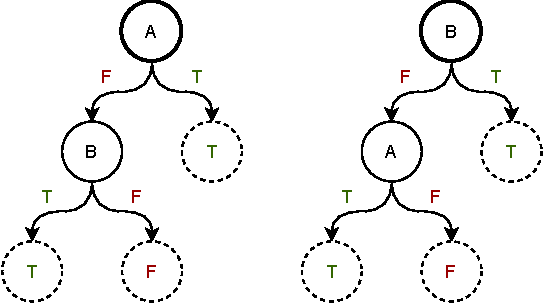
\includegraphics[scale = 0.9]{img/dt1.pdf}
  \end{figure}
\end{esempio}
Essendo sempre nel concept learning, nel caso di funzioni booleane, anche il
target è booleano.
\begin{teorema}
  Con un albero decisionale posso rappresentare tutte le
  funzioni booleane
\end{teorema}
\begin{proof}
  Prendiamo una qualsiasi funzione booleana e la traduciamo in tabella di
  verità.\\
  A partire dalla tabella costruisco l'albero decisionale dove ogni percorso
  radice-foglia è un esempio (quindi una riga) della tabella di verità.\\
  Dato che ogni funzione booleana può essere rappresentata con una tabella di
  verità posso costruire un albero decisionale per qualsiasi funzione booleana.
\end{proof}
Il metodo appena descritto comunque dimostra il teorema ma non è sempre
efficiente, dovendo memorizzare tutto.
\begin{teorema}
  Avendo una funzione booleana con $n$ attributi allora posso costruire una
  tabella di verità con $2^n$ righe. Inoltre posso costruire potenzialmente
  $2^{2^n}$ diverse ma con lo stesso significo, e quindi altrettanti alberi
  decisionali.
\end{teorema}
Vediamo quindi un algoritmo generale per la costruzione dell'albero:
\begin{enumerate}
  \item si inizia con un albero vuoto
  \item scelgo un attributo opportuno per fare lo \textit{split} dei dati
  \item per ogni \textit{split} dell'albero:
  \begin{itemize}
    \item se non c'è altro da fare si fa la predizione con l'ultimo nodo foglia
    \item altrimenti si torna allo step 2 e si procede con un altro
    \textit{split}
  \end{itemize}
\end{enumerate}
Bisognerà capire:
\begin{itemize}
  \item come fare in modo ottimizzato lo `\textit{split}
  \item quando fermare la costruzione (quindi capire quando ``non c'è altro da
  fare'')
\end{itemize}
\begin{esempio}
  Prendiamo il solito esempio giocattolo di quando andare a fare sport in base
  al clima.\\
  In base al valore di \textit{outlook} ottengo tre tabelle, in base al valore
  di overcast, con target $play$ (nell'immagine il terzo arco è etichettato con
  $rainy$ e non con $text$):
  \begin{figure}[H]
    \centering
    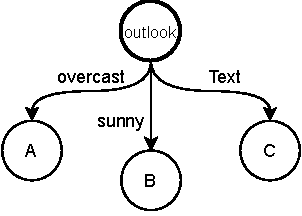
\includegraphics[scale = 0.9]{img/dt2.pdf}
  \end{figure}
  \begin{table}[H]
    \centering
    \begin{tabular}{c|c|c|c|c}
      outlook & temp & humidity & windy & play\\
      \hline
      overcast & H & H & $\bot$ & \color{darkgreen}{yes}\\
      overcast & C & N & $\top$ & \color{darkgreen}{yes}\\
      overcast & M & H & $\top$ & \color{darkgreen}{yes}\\
      overcast & H & N & $\bot$ & \color{darkgreen}{yes}
    \end{tabular}
    \caption{Tabella A}
  \end{table}
  \begin{table}[H]
    \centering
    \begin{tabular}{c|c|c|c|c}
      outlook & temp & humidity & windy & play\\
      \hline
      sunny & H & H & $\bot$ & \color{red}{no}\\
      sunny & H & H & $\top$ & \color{red}{no}\\
      sunny & M & H & $\bot$ & \color{red}{no}\\
      sunny & C & N & $\bot$ & \color{darkgreen}{yes}\\
      sunny & M & N & $\top$ & \color{darkgreen}{yes}
    \end{tabular}
    \caption{Tabella B}
  \end{table}
  \begin{table}[H]
    \centering
    \begin{tabular}{c|c|c|c|c}
      outlook & temp & humidity & windy & play\\
      \hline
      rainy & M & H & $\bot$ & \color{darkgreen}{yes}\\
      rainy & C & N & $\bot$ & \color{darkgreen}{yes}\\
      rainy & C & N & $\top$ & \color{red}{no}\\
      rainy & M & N & $\bot$ & \color{darkgreen}{yes}\\
      rainy & M & H & $\top$ & \color{red}{no}
    \end{tabular}
    \caption{Tabella C}
  \end{table}
  Dividendo tramite i valori di outlook ho fatto uno \textit{split}, dividendo
  così i dati.\\
  Vediamo un secondo i valori del target nei vari casi:
  \begin{itemize}
    \item nel caso di \textit{overcast} ho 4 \textit{yes} e 0 \textit{no}
    \item nel caso di \textit{sunny} ho 2 \textit{yes} e 3 \textit{no}
    \item nel caso di \textit{rainy} ho 3 \textit{yes} e 2 \textit{no}
  \end{itemize}
  Posso quindi usare una \textbf{funzione di costo} per fissare quando una
  distribuzione è omogenea (come nel caso di \textit{overcast}) o quando no (gli
  altri due casi). Lo \textit{split} infatti andrebbe fatto in base ai valori
  del target, più sono omogenei e meglio è, in quanto nel momento in cui si
  presenta un nuovo test per la classificazione con \textit{outlook} pari a
  \textit{overcast} saprò già cosa fare (in quanto nello storico delle
  esperienze ho sempre avuto \textit{yes}). Le altre due situazioni sono
  ambigue e quindi, in quei due casi, devo procedere con la costruzione
  dell'albero per ottenere informazioni cercando di rimuovere l'incertezza.  
\end{esempio}
La \textbf{funzione costo} è alla base della strategia della costruzione
dell'albero.\\
Una strategia può essere quella ``a maggioranza'', prendendo l'attributo che con
i suoi valori ha meno disomogeneità. Per farlo calcolo la differenza tra $yes$ e
$no$ di ogni valore per un certo attributo, sommandone io risultati. Scelgo
l'attributo con più omogeneità (e quindi somma più bassa), che ha una
distribuzione più pulita dei risultati. Se ho valori con solo
$yes$ o solo $no$ sommo 0.
\begin{esempio}
  Prendendo le tre tabelle sopra, per \textit{outlook} avrei:
  \[0+1+1=2\]
  Se avessi avuto un attributo con:
  \begin{itemize}
    \item primo valore: 1 \textit{yes} e 1 \textit{no}
    \item secondo valore: 2 \textit{yes} e 0 \textit{no}
    \item terzo valore: 0 \textit{yes} e 4 \textit{no}
    \item quarto valore: 2 \textit{yes} e 4 \textit{no}
    \item quinto valore: 2 \textit{yes} e 2 \textit{no} 
  \end{itemize}
  avrei avuto:
  \[1+0+0+2+2=5\]
\end{esempio}
Gli alberi di decisione possono essere utilizzati anche nel continuo, per
attributi numerici.
\begin{esempio}
  Prendiamo le istanze definite da due attributi, $x$ e $y$ e costruisco un
  albero di decisione che definisce in quali aree del piano ho $-$ e quali ho
  $+$.
  \newpage
  Si ha il seguente piano (\textbf{sull'asse delle $y$ il primo valore a partire
  dall'origine è un 5 non un 7}): 
  \begin{figure}[H]
    \centering
    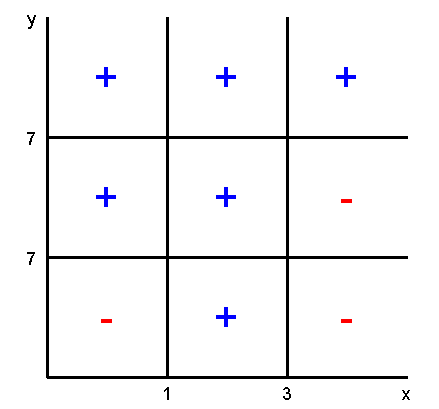
\includegraphics[scale = 0.8]{img/dt3.pdf}
  \end{figure}
  E si ottiene, per esempio, il seguente albero decisionale:
  \begin{figure}[H]
    \centering
    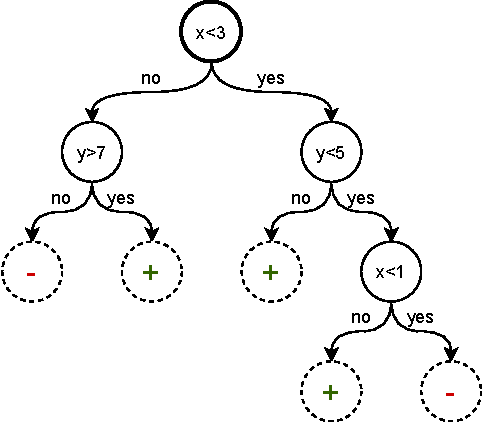
\includegraphics[scale = 0.9]{img/dt4.pdf}
  \end{figure}
  Dove a ciascun nodo è associata una condizione e agli archi il fatto che sia
  verificata o meno.\\
  Si nota come non si hanno tutte le condizioni, infatti, per esempio, con $x>3$
  mi basta $y>7$ per trovare il $+$ e $y<7$ per il $-$ (non dovendo andare
  specificatamente a guardare anche $y<5$ o $y>5$).\\
  \textbf{Quello disegnato è solo uno dei possibili alberi.}
\end{esempio}
\subsection{Algoritmo ID3}
Vista la difficoltà di scegliere l'albero si ha l'idea di scegliere un piccolo
albero di partenza (o più piccoli) e ricorsivamente l'attributo più
significativo (sia nei nodi rossi intermedi che nelle foglie) come radice per il
sotto-albero. Si fanno quindi crescere in modo 
coerente gli alberi piccoli scelti in partenza. Si punta ad arrivare ad un
albero valido per tutti gli esempi ricevuti e anche per quelli non visti.\\
Iniziamo a vedere l'algoritmo anche se saranno necessarie molte specifiche:
\begin{algorithm}[H]
  \begin{algorithmic}
    \Function{ID3}{}
    \State $A \gets$ \textit{il ``miglior'' attributo di decisione per il
    prossimo nodo}
    \State \textit{assegno A come attributo di decisione per il nodo, che sarà
    rosso}
    \For {\textit{ogni valore dell'attributo A}}
    \State \textit{creo un discendente}
    \EndFor
    \State \textit{ordina gli esempi di training alla foglia}
    \State \textit{in base al valore dell'attributo del branch}
    \If {\textit{ho classificato tutti gli esempi di training}}
    \State \textit{mi fermo}
    \Else
    \State \textit{itero sulle foglie appena create}
    \EndIf
    \EndFunction
  \end{algorithmic}
  \caption{Algoritmo ID3 (Iterative Dichotomiser 3)}
\end{algorithm}
Il \textbf{bias induttivo} su ID3 è che preferisce alberi piccoli.\\
Bisogna in primis capire cosa si intende come \textbf{attributo migliore}. Per
farlo introduciamo la seguente notazione:
\[[esempi\,\,\,positivi+,\,\,esempi\,\,\,negativi-]\]
entrambi rappresentati con un valore intero. Gli esempi positivi sono gli esempi
che già mi hanno restituito \textit{yes} mentre quelli negativi. In generale
sono tutti esempi su cui devo ancora valutare l'attributo. E proseguo così
assegnando etichette positive e negative.
Vediamo quanto detto:

\begin{figure}[H]
  \centering
  \begin{tikzpicture}[nodes={draw}, -, sibling distance=70pt, level
    distance=30pt]  
    \node{\color{red} $A_1=\,?$ \color{black} [29+, 35-]}
    child { node {\color{blue} True}
      child{ node {\color{orange} [21+, 5-]}}}
    child { node {\color{blue} False}
      child{ node {\color{orange} [8+, 30-]}}};
  \end{tikzpicture}
\end{figure}

Se siamo nella situazione in cui dobbiamo confrontare l'attributo sopra con un
altro, per esempio:
\begin{figure}[H]
  \centering
  \begin{tikzpicture}[nodes={draw}, -, sibling distance=70pt, level
    distance=30pt]  
    \node{\color{red} $A_2=\,?$ \color{black} [29+, 35-]}
    child { node {\color{blue} True}
      child{ node {\color{orange} [18+, 33-]}}}
    child { node {\color{blue} False}
      child{ node {\color{orange} [11+, 2-]}}};
  \end{tikzpicture}
\end{figure}
Entrambe le foglie del primo attributi ci parlano di valori sbilanciati (tra
esempi positivi e negativi), a differenza delle due del secondo attributo, dove
sono una sbilanciata e una no. Per ora stabiliamo ad occhio lo sbilanciamento.\\
Il criterio di scelta ci porta a preferire lo sbilanciamento, verso un ideale
``tutti positivi'' o ``tutti negativi''. Quindi se un attributo ha divisioni
sbilanciate è da ritenersi migliore.\\ 
Per essere ancora più precisi bisogna richiamare la matematica
dell'\textbf{entropia}.
\begin{definizione}
  Dato un training set $S$ con valori $v_i,\,\,i=1\ldots n$. Se l'entropia di un
  insieme di bit misura più o meno la sua quantità di informazione (quanto è
  ``speciale'') noi possiamo richiamare una formula per l'entropia su S:
  \[I(P(v_1),\ldots,P(v_n))=\sum_{i=1}-P(v_i)\log_2P(v_i)\]
  Dove $I(x)$ indica il valore dell'entropia su $x$ e $P(y)$ sta per la
  probabilità legata ad un valore $y$.  \\
  Nel caso booleano le istanze presenti in un certo insieme $S$ sono associate
  ad un'etichetta, conteggiandole. Nella variabile $p$ conto i valori di $S$ con
  etichetta positiva e con $n$ negativa (esempi positivi e negativi). Ottengo
  quindi in modo esplicito la sommatoria:
  \[I\left(\frac{p}{p+n},\frac{n}{p+n}\right)=-\frac{p}{p+n}\log_2\frac{p}{p+n}
    -\frac{n}{p+n}\log_2\frac{n}{p+n}\]  
  Se inoltre diciamo che $p_+$ è la proporzione di esempi positivi e $p_-$ di
  quelli negativi (saranno quindi tra 0 e 1) possiamo misurare
  l'\textbf{impurità} di $S$ con l'entropia: 
  \[Entropy(S)=-p_+\log_2 p_+-p_-\log_2 p_-\]
  Avrò quindi alta entropia se positivi e negativi sono ``metà e metà''
\end{definizione}
Parliamo quindi di \textbf{information gain} $IG$ che viene calcolato su ogni
attributo $A$ e su $S$:
\[IG(S,A)=I\left(\frac{p}{p+n},\frac{n}{p+n}\right)-remainder(A)\]
dove:
\[remainder(A)=\sum_{i=1}^v \frac{p_i+n_i}{p+n}
  I\left(\frac{p_i}{p_i+n_i},\frac{n_i}{p_i+n_i}\right)\]
e quindi l'information gain è la riduzione aspettata nell'entropia per ordinare
$S$ sull'attributo $A$. Si sceglie l'attributo con il maggiore IG.\\
Possiamo riscrivere il conto come:
\[IG(S,A)=Entropy(S)-\sum_{v\in values(A)}\frac{|S_v|}{|S|}Entropy(S_v)\]
\begin{esempio}
  Vediamo l'esempio di calcolo di entropia di $A_1$ con [29+,35-]:
  \[Entropy([29+,35-])=
    -\frac{29}{64}\log_2\frac{29}{64}-\frac{35}{64}\log_2\frac{35}{64}=0.99\]
  Calcolo anche l'information gain di $A_1$, sapendo che
  $Entropy([21+,5-])=0.71$ e $Entropy([8+,30-])=0.74$,
  e quindi:
  \[IG(S,A_1)=0.99-\frac{26}{64}\cdot 0.71-\frac{38}{64}\cdot 0.74=0.27\]
  ugualmente calcolo $IG(S,A_2)=0.12$. \\
  Quindi so che devo scegliere $A_1$ in quanto $0.27 > 0.12$
\end{esempio}
Facciamo qualche osservazione finale sull'\textbf{algoritmo ID3}:
\begin{itemize}
  \item lo spazio delle ipotesi è completo e sicuramente contiene il target
  \item ho in output una singola ipotesi
  \item non si ha backtracking sugli attributi selezionati, si procede con una
  ricerca greedy (ma trovo scelte buone localmente e non ottime)
  \item fa scelte basate su una ricerca statistica, facendo sparire incertezze
  sui dati
  \item il bias non è sulla classe iniziale, essendo lo spazio delle ipotesi
  completo, ma sulla scelta di solo alcune funzioni, preferendo alberi corti (e
  più semplici) e posizionando attributi ad alto information gain vicino alla
  radice. Il bias è quindi sulla preferenza di alcune ipotesi. Si usa il
  criterio euristico di \textit{rasoio di Occam}
  \item $H$ è l'insieme potenza delle istanze $X$
\end{itemize}
Viene introdotto però l'\textbf{overfitting}.
\begin{definizione}
  \textit{Definizione tratta da wikipedia.}\\
  Definiamo formalmente l'\textbf{overfitting} come l'adattamento eccessivo,
  ovvero quando 
  un un modello statistico molto complesso si adatta al campione perché ha un
  numero eccessivo di parametri rispetto al numero di osservazioni. SI ha
  quindi che un modello assurdo e sbagliato può adattarsi perfettamente se è
  abbastanza complesso rispetto alla quantità di dati disponibili.\\
  Nel machine learning se il learner viene addestrato troppo a lungo il modello
  potrebbe adattarsi a caratteristiche che sono specifiche solo del training
  set, ma che non hanno riscontro nel resto dei casi quindi le prestazioni sui
  dati non visionati saranno drasticamente peggiori.\\
  L'opposto è l'\textbf{underfitting}.
\end{definizione}

Se misuro l'errore di una ipotesi
$h$ sul training set ($error_{traini}(h)$) e poi misuro l'errore di quella
ipotesi sull'intero set delle possibili istanze
$D$ ($error_D(h)$) ho che l'ipotesi $h$ va in \textbf{overfit} sul quel data set
se:
\[error_{traini}(h) < error_{traini}(h') \,\,\land
  \,\,error_D(h)>error_D(h')\]
quindi se presa un'altra ipotesi questa è migliore della prima e ha un errore
sull'intera distribuzione delle ipotesi inferiore vado in \textit{overfit}. Il
problema è che non posso sapere se esiste tale $h'$. Per evitare il problema uso
sempre il rasoio di Occam scegliendo ipotesi semplici ed evitando di far
crescere l'albero quando lo ``split'' non è statisticamente significativo. Un
altro modo è quello di togliere pezzi, all'albero, che toccano poche istanze o
pure calcolare una \textit{misura di complessità dell'albero}, minimizzando la
grandezza dell'albero e gli errori del \textit{training set}, usando il
\textbf{Minimum Description Length (\textit{MDL})}.\\
In ID3 quindi posso scegliere sia in base all'\textit{information gain} massimo
o all'\textit{entropia} minima tra gli attributi.
\subsubsection{Esercitazione su ID3}
Quando parliamo di \textit{entropia} stiamo volgendo un esperimento
concettuale. Prima dell'esperimento si ha una certa incertezza su un certo
eventi, che sparisce, con sorpresa, una volta eseguito l'esperimento se l'evento
accade. D'altro canto qualora accade un evento atteso siamo meno sorpresi del
fatto. Nel primo caso però si ritiene di ottenere molta informazione, nel
secondo caso poca. Come se ponessimo in una vasca quattro palline rosse, non
sarei stupito di estrarne una rossa, essendo quello che mi aspetto. D'altro
canto se ne aggiungo quattro verdi l'estrazione sarà inattesa e quindi più
interessante.\\ 
Si cerca un modo di quantificare questa ``sorpresa''. Riprendendo l'esempio
della palline posso dire che nel primo caso (solo rosse) ho \textbf{bassa
  entropia} e nel secondo caso (palline miste) \textbf{alta entropia}. Un caso
intermedio sarebbe a \textbf{media entropia}.\\
Quindi, detta $P(x)$ la probabilità che avvenga un evento $x$ e con $I(p)$
l'informazione che ottengo dopo che l'evento si è verificato:
\begin{itemize}
  \item $P(x)=1\to I(p)=0$
  \item $P(x)=0\to I(p)=\infty$
\end{itemize}
L'informazione $I(p)$ e quindi una quantità non negativa:
\[I(p)\geq 0\]
Definiamo quindi l'informazione, detta anche \textit{self-information}, per un
evento $E$: 
\[I(E)=-\log_2(P(E))\]
Inoltre ho che è additiva se gli eventi sono indipendenti, ovvero:
\[I(p_1,p_2)=I(p_1)+I(p_2)\]
Bisogna però estendere l'informazione a tutte le possibili distribuzioni di
tutti i possibili esiti che ho in un esperimento concettuale.\\
Passiamo quindi alle definizioni matematiche per l'\textbf{entropia}:
\begin{itemize}
  \item $X\sim P_X$, presa una certa variabile $X$ dell'esperimento con una
  certa funzione di probabilità associata $P_X$
  \item $Val(X)=\{x_1,\ldots,x_n\}$, ovvero il range di valori della variabile
  $X$
  \item $p_i=P_X(x_i)$, probabilità per quel valore della variabile $X$
  \item $g:\mathbb{R}\to\mathbb{R}$ una funzione arbitraria tale per cui $g(X)$
  è una variabile causale. Si definisce l'aspettativa di $G(X)$ su $P$ come:
  \[E_P[g(X)]=\sum_{x\in Val(X)} g(x)\cdot P_X(x)\]
\end{itemize}
Giungendo quindi alla formula dell'\textbf{entropia} di una variabile:
\[H[X]=-\sum_{i=1}^n p_i\cdot\log_2 p_i=E_P[\log_2(p)]\]
Quindi:
\begin{definizione}
  L'\textbf{entropia}, definita da Claude Shannon (e quindi spesso chiamata
  \textbf{entropia di Shannon}), è l'informazione media associata ad
  una distribuzione di probabilità.
\end{definizione}
Vediamo un esempio:
\begin{esempio}
  Suppongo di lanciare una moneta, si ha:
  \[P(testa)=P(croce)=\frac{1}{2}\]
  Definiamo che testa è specificata da $X=0$ e croce da $X=1$.\\
  Calcoliamo quindi:
  \[H(p)=-p(0)\cdot \log_2 p(0)-p(1)\cdot\log_2
    p(1)=-2\cdot(\frac{1}{2}\cdot\log_2\frac{1}{2})=1\] 
  Una moneta ``onesta'' ha quindi entropia pari a 1 (avendo due probabili esiti
  equiprobabili non ho certezza del risultato).\\
  Ipotizziamo di avere una moneta magica che cade solo sulla testa (quindi
  $P(0)=1$ e $P(1)=0$:
  \[H(p)=-p(0)\cdot \log_2 p(0)-p(1)\cdot\log_2 p(1)=-\log_2 (1)=0\]
  Una moneta ``non onesta'' ha quindi entropia pari a 0 (ho infatti certezza del
  risultato).
\end{esempio}
\begin{esempio}
  Considero il seguente training set, con 4 esempi e target $T$:
  \begin{table}[H]
    \centering
    \begin{tabular}{c|c|c|c|c|c}
      example & A & B & C & D & T\\
      \hline
      $x_1$ & 0 & 0 & 1 & 1 & \color{darkgreen}{1}\\
      $x_2$ & 0 & 1 & 1 & 1 & \color{darkgreen}{1}\\
      $x_3$ & 0 & 1 & 0 & 0 & \color{red}{0}\\
      $x_4$ & 0 & 1 & 0 & 1 & \color{darkgreen}{1}\\
    \end{tabular}
  \end{table}
  Si ha quindi la seguente distribuzione di probabilità relativa al target
  (avendo un \textit{no} e tre \textit{yes}):
  \[P_T=\left[\frac{1}{4},\frac{3}{4}\right]\]
  e quindi posso calcolare l'entropia della tabella:
  \[H(P_T)=-P_T(0)\cdot \log_2 P_T(0)-P_T(1)\cdot\log_2
    P_T(1)=-\frac{1}{4}\cdot\log_2\frac{1}{4}-\frac{3}{4}\cdot\log_2
    \frac{3}{4}= 0.81\]
  La tabella può essere vista come un risultato di un esperimento concettuale.
\end{esempio}
\begin{definizione}
  Definiamo l'\textbf{entropia di una distribuzione condizionale}. Presa $X$
  come una variabile discreta arbitraria con valori $\{x_1,\ldots,x_n\}$, che
  hanno ciascuno probabilità $P_X(x_i)$ ho che, per la distribuzione
  condizionale:
  \[P{Y|X=x_i}(y_j)=P_{Y|X}(y_j|x_i)\]
  Ovvero la distribuzione dei valori della variabile $Y$ dato $X=x_i$.\\
  Quindi voglio sapere la probabilità di $Y$ condizionata da un esperimento
  precedente su $X$.\\
  Per l'entropia ho:
  \[H_{Y|X=x_i}=-\sum_{j=1}^m P_{Y|X}(y_j|x_i)\cdot \log_2 P_{Y|X}(y_j|x_i)\]
  quindi è la solita formula ma con la probabilità condizionale.
\end{definizione}
\begin{definizione}
  Definiamo \textbf{entropia condizionale} come il valore medio, ovvero il
  valore atteso, dell'entropia di $p_{Y|X=x_i}$ per ciascun valore di $X$ che
  condiziona $Y$, ovvero:
  \[H_{Y|X}=\sum_{i=1}^n P_X(x_i)H_{Y|X=x_i}\]
  ottenendo l'\textbf{entropia condizionale}:
  \[H[Y|X]=\sum P(x)\cdot H(Y|X=x)\]
\end{definizione}
\begin{esercizio}
  Considero il seguente training set, con 4 esempi e target $T$:
  \begin{table}[H]
    \centering
    \begin{tabular}{c|c|c|c|c|c}
      example & A & B & C & D & T\\
      \hline
      $x_1$ & 0 & 0 & 1 & 1 & \color{darkgreen}{1}\\
      $x_2$ & 0 & 1 & 1 & 1 & \color{darkgreen}{1}\\
      $x_3$ & 0 & 1 & 0 & 0 & \color{red}{0}\\
      $x_4$ & 0 & 1 & 0 & 1 & \color{darkgreen}{1}\\
    \end{tabular}
  \end{table}
  Abbiamo già calcolato l'entropia associabile al valore target $H[P_T]=0.81$.\\
  Passiamo ora all'uso di ID3 per la costruzione dell'albero.\\
  Dobbiamo cercare gli split corretti tramite information gain, usando
  l'entropia condizionale.\\
  Partiamo con il primo attributo: $A$. Si ha che $P_A(0)=1$ e $P_A(1)=0$,
  quindi:
  \[H[T|A=0]=-p_{T|A}(0|0)\cdot \log_2(p_{T|A}(0|0))-p_{T|A}(1|0)\cdot
    \log_2(p_{T|A}(1|0))=\]
  \[-\frac{1}{4}\cdot\log_2\frac{1}{4}-
    \frac{3}{4}\cdot\log_2\frac{3}{4}=0.81\]
  (Risultato pari a quello dell'intero training set in quanto $A$ è sempre 0)\\
  Non devo calcolare $H[T|A=1]$ in quanto $A$ non è mai pari ad 1.\\
  Inoltre si ha:
  \[H[T|A]=P_A(0)\cdot H[T|A=0]+P_A(1)\cdot H[T|A=1]=1\cdot 0.81=0.81\]
  Posso quindi calcolare l'\textit{information gain}:
  \[IG[T;A]=H[T]-H[T|A]=0.81-0.81=0\]
  Quindi per $A$ ho la seguente distribuzione del target (avendo nel target 3
  esempi positivi e uno negativo e $A$ sempre con valore 0):
  \begin{figure}[H]
    \centering
    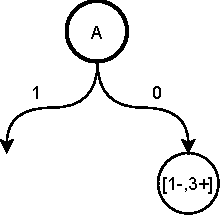
\includegraphics[scale = 0.9]{img/id1.pdf}
  \end{figure}
 \textbf{\textit{Ricordiamo che ID3 sceglie per lo splitting l'attributo che
     rende massimo l'information gain.}}\\
  Passo quindi all'attributo $B$. Si ha che $P_B(0)=\frac{1}{4}$ e
  $P_B(1)=\frac{3}{4}$, quindi:
  \[H[T|B=0]=-p_{T|B}(0|0)\cdot \log_2(p_{T|B}(0|0))-p_{T|B}(1|0)\cdot
    \log_2(p_{T|B}(1|0))=\]
  \[-0\cdot \log_2 0-1\cdot \log_2 1=0\]
  e:
  \[H[T|B=1]=-p_{T|B}(0|1)\cdot \log_2(p_{T|B}(0|1))-p_{T|B}(1|1)\cdot
    \log_2(p_{T|B}(1|1))=\]
  \[-\frac{1}{3}\cdot\log_2\frac{1}{3}-
    \frac{2}{3}\cdot\log_2\frac{2}{3}=0.91\]
  (ho quindi una partizione migliore con $B=0$)\\
  Inoltre si ha:
  \[H[T|B]=P_B(0)\cdot H[T|B=0]+P_B(1)\cdot H[T|B=1]=\frac{1}{4}\cdot
    0+\frac{3}{4}\cdot 0.91=0.68\]
  Posso quindi calcolare l'\textit{information gain}:
  \[IG[T;B]=H[T]-H[T|B]=0.81-0.68=0.13\]
  Quindi per $B$ ho:
  \begin{figure}[H]
    \centering
    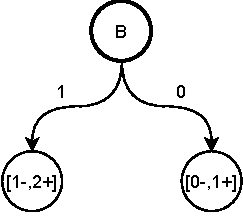
\includegraphics[scale = 0.9]{img/id2.pdf}
  \end{figure}
  Ho quindi un partizionamento più interessante.\\
  Passo quindi all'attributo $C$. Si ha che $P_C(0)=\frac{1}{2}$ e
  $P_C(1)=\frac{1}{2}$, quindi:
  \[H[T|C=0]=-p_{T|C}(0|0)\cdot \log_2(p_{T|C}(0|0))-p_{T|C}(1|0)\cdot
    \log_2(p_{T|C}(1|0))=\]
  \[-\frac{1}{2}\cdot \log_2 \frac{1}{2}-\frac{1}{2}\cdot \log_2 \frac{1}{2}=1\]
  e:
  \[H[T|C=1]=-p_{T|C}(0|1)\cdot \log_2(p_{T|C}(0|1))-p_{T|C}(1|1)\cdot
    \log_2(p_{T|C}(1|1))=\]
  \[-0\cdot \log_2 0-1\cdot \log_2 1=0\]
  Inoltre si ha:
  \[H[T|C]=P_C(0)\cdot H[T|C=0]+P_C(1)\cdot H[T|C=1]=\frac{1}{2}\cdot
    1+\frac{1}{2}\cdot 0=\frac{1}{2}\]
  Posso quindi calcolare l'\textit{information gain}:
  \[IG[T;C]=H[T]-H[T|C]=0.81-\frac{1}{2}=0.31\]
  Quindi per $C$ ho:
  \begin{figure}[H]
    \centering
    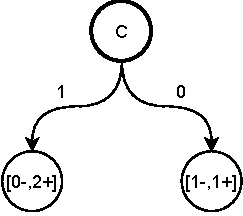
\includegraphics[scale = 0.9]{img/id3.pdf}
  \end{figure}
  $C$ migliora ancora il partizionamento.\\
  Passo quindi all'attributo $D$. Si ha che $P_D(0)=\frac{1}{4}$ e
  $P_D(1)=\frac{3}{4}$, quindi:
  \[H[T|D=0]=-p_{T|D}(0|0)\cdot \log_2(p_{T|D}(0|0))-p_{T|D}(1|0)\cdot
    \log_2(p_{T|D}(1|0))=\]
  \[-1\cdot \log_2 1-0\cdot \log_2 0=0\]
  e:
  \[H[T|D=1]=-p_{T|D}(0|1)\cdot \log_2(p_{T|D}(0|1))-p_{T|D}(1|1)\cdot
    \log_2(p_{T|D}(1|1))=\]
  \[-0\cdot \log_2 0-1\cdot \log_2 1=0\]
  Inoltre si ha:
  \[H[T|D]=P_D(0)\cdot H[T|D=0]+P_D(1)\cdot H[T|D=1]=\frac{1}{4}\cdot
    0+\frac{3}{4}\cdot 0=0\]
  Posso quindi calcolare l'\textit{information gain}:
  \[IG[T;D]=H[T]-H[T|D]=0.81-0=0.81\]
  Quindi per $D$ ho:
  \begin{figure}[H]
    \centering
    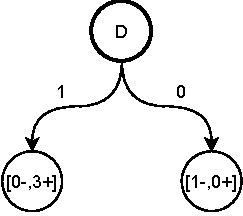
\includegraphics[scale = 0.9]{img/id4.pdf}
  \end{figure}
  $D$ rende quindi il massimo della ``purezza'' tra i valori di $D$ e quelli del
  target. Non ho incertezza nel partizionamento.\\
  Quindi, ricapitolando, ho i seguenti information gain:
  \begin{itemize}
    \item $IG[T;A]=0$
    \item $IG[T;B]=0.13$
    \item $IG[T;C]=0.31$
    \item $IG[T;D]=0.81$, \textbf{che è il valore massimo} e che rende minima la
    ``sorpresa''
  \end{itemize}
\end{esercizio}
\begin{esercizio}
  Considero il seguente training set, con 4 esempi e target $T$:
  \begin{table}[H]
    \centering
    \begin{tabular}{c|c|c|c|c|c}
      example & A & B & C & D & T\\
      \hline
      $x_1$ & 0 & 0 & 1 & $\ldots$ & \color{darkgreen}{1}\\
      $x_2$ & 0 & 1 & 1 & $\ldots$ & \color{darkgreen}{1}\\
      $x_3$ & 0 & 1 & 0 & $\ldots$ & \color{red}{0}\\
      $x_4$ & 0 & 1 & 0 & $\ldots$ & \color{darkgreen}{1}\\
    \end{tabular}
  \end{table}
  Bisogna riempire $D$ per rendere massimo l'information gain.
  \newpage
  Per farlo basta mettere gli stessi valori del target, in modo che sia
  l'attributo che meglio distribuisca i valori del target, ottenendo quindi lo
  stesso training set dell'esercizio precedente:
  \begin{table}[H]
    \centering
    \begin{tabular}{c|c|c|c|c|c}
      example & A & B & C & D & T\\
      \hline
      $x_1$ & 0 & 0 & 1 & 1 & \color{darkgreen}{1}\\
      $x_2$ & 0 & 1 & 1 & 1 & \color{darkgreen}{1}\\
      $x_3$ & 0 & 1 & 0 & 0 & \color{red}{0}\\
      $x_4$ & 0 & 1 & 0 & 1 & \color{darkgreen}{1}\\
    \end{tabular}
  \end{table}
  Un'alternativa è l'esatto opposto, in quanto otterrei la stessa
  ridistribuzione del target, rimuovendo ogni ``sorpresa'' ulteriore ma
  lasciando solo quella della tabella iniziale:
  \begin{table}[H]
    \centering
    \begin{tabular}{c|c|c|c|c|c}
      example & A & B & C & D & T\\
      \hline
      $x_1$ & 0 & 0 & 1 & 0 & \color{darkgreen}{1}\\
      $x_2$ & 0 & 1 & 1 & 0 & \color{darkgreen}{1}\\
      $x_3$ & 0 & 1 & 0 & 1 & \color{red}{0}\\
      $x_4$ & 0 & 1 & 0 & 0 & \color{darkgreen}{1}\\
    \end{tabular}
  \end{table}
\end{esercizio}
\begin{esercizio}
  Considero il seguente training set, con 4 esempi e target $T$:
  \begin{table}[H]
    \centering
    \begin{tabular}{c|c|c|c|c}
      example & $f_1$ & $f_2$ & $f_3$ & T\\
      \hline
      $x_1$ & 1 & 1 & 1 & \color{darkgreen}{1}\\
      $x_2$ & 0 & 1 & 1 & \color{red}{0}\\
      $x_3$ & 0 & 0 & 1 & \color{darkgreen}{1}\\
      $x_4$ & 0 & 0 & 0 & \color{red}{0}\\
    \end{tabular}
  \end{table}
  Vogliamo completare il seguente albero decisionale:
  \begin{figure}[H]
    \centering
    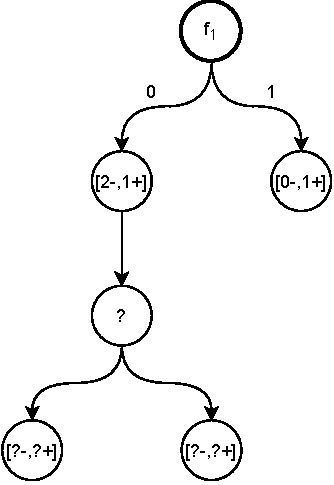
\includegraphics[scale = 0.75]{img/id5.pdf}
  \end{figure}
  Partendo da $f_1$ so che se arriva un nuovo esempio non potrò proseguire da
  $[0-,1+]$ in quanto so già che in quel caso avrei un'istanza positiva, valore
  minimo $0$.\\
  Quindi se $f_1=0$ vado a scegliere un nuovo attributo in quanto ancora non ho
  una distribuzione certa. Considero quindi le righe in cui $f_1=0$ e avanzo
  iterativamente studiando $f_2$ ed $f_3$. Studio quindi il sottoinsieme: 
  \begin{table}[H]
    \centering
    \begin{tabular}{c|c|c|c}
      example  & $f_2$ & $f_3$ & T\\
      \hline
      $x_2$ & 1 & 1 & \color{red}{0}\\
      $x_3$ & 0 & 1 & \color{darkgreen}{1}\\
      $x_4$ & 0 & 0 & \color{red}{0}\\
    \end{tabular}
  \end{table}
  e avanzo fino a che non finisco gli attributi (o arrivo in un punto in cui,
  come per il ramo 1 di $f_1$ non posso più continuare).\\
  Per questo nuovo sottoinsieme calcolo:
  \[P_T=\left[\frac{2}{3},\frac{1}{4}\right]\]
  e quindi posso calcolare l'entropia della tabella:
  \[H(P_T)=-P_T(0)\cdot \log_2 P_T(0)-P_T(1)\cdot\log_2
    P_T(1)=-\frac{2}{3}\cdot\log_2\frac{2}{3}-\frac{1}{3}\cdot\log_2
    \frac{1}{3}= 0.91\]
  Passo quindi all'attributo $f_2$. Si ha che $P_{f_2}(0)=\frac{2}{3}$ e
  $P_{f_2}(1)=\frac{1}{3}$, quindi:
  \[H[T|f_2=0]=-p_{T|f_2}(0|0)\cdot \log_2(p_{T|f_2}(0|0))-p_{T|f_2}(1|0)\cdot
    \log_2(p_{T|f_2}(1|0))=\]
  \[-\frac{1}{2}\cdot \log_2 \frac{1}{2}-\frac{1}{2}\cdot \log_2 \frac{1}{2}=1\]
  e:
  \[H[T|f_2=1]=-p_{T|f_2}(0|1)\cdot \log_2(p_{T|f_2}(0|1))-p_{T|f_2}(1|1)\cdot
    \log_2(p_{T|f_2}(1|1))=\]
  \[-0\cdot \log_2 0-1\cdot \log_2 1=0\]
  Inoltre si ha:
  \[H[T|f_2]=P_{f_2}(0)\cdot H[T|f_2=0]+P_{f_2}(1)\cdot
    H[T|f_2=1]=\frac{2}{3}\cdot 1+\frac{1}{3}\cdot 0=\frac{2}{3}\]
  Posso quindi calcolare l'\textit{information gain}:
  \[IG[T;f_2]=H[T]-H[T|f_2]=0.81-\frac{2}{3}=0.25\]
  
  Passo quindi all'attributo $f_3$. Si ha che $P_{f_3}(0)=\frac{1}{3}$ e
  $P_{f_3}(1)=\frac{2}{3}$, quindi:
  \[H[T|f_3=0]=-p_{T|f_3}(0|1)\cdot \log_2(p_{T|f_3}(0|1))-p_{T|f_3}(1|1)\cdot
    \log_2(p_{T|f_3}(1|1))=\]
  \[-1\cdot \log_2 1-0\cdot \log_2 0=0\]
  e:
  \[H[T|f_3=1]=-p_{T|f_3}(0|0)\cdot \log_2(p_{T|f_3}(0|0))-p_{T|f_3}(1|0)\cdot
    \log_2(p_{T|f_3}(1|0))=\]
  \[-\frac{1}{2}\cdot \log_2 \frac{1}{2}-\frac{1}{2}\cdot \log_2 \frac{1}{2}=1\]
  Inoltre si ha:
  \[H[T|f_3]=P_{f_3}(0)\cdot H[T|f_3=0]+P_{f_3}(1)\cdot
    H[T|f_3=1]=\frac{1}{3}\cdot 0+\frac{2}{3}\cdot 1=\frac{2}{3}\]
  Posso quindi calcolare l'\textit{information gain}:
  \[IG[T;f_3]=H[T]-H[T|f_3]=0.81-\frac{2}{3}=0.25\]
  Avendo $f_1$ e $f_2$ lo stesso $IG$ prendo il primo e quindi ho:
  \begin{figure}[H]
    \centering
    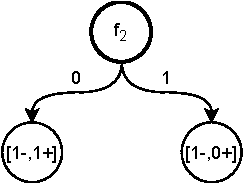
\includegraphics[scale = 0.9]{img/id6.pdf}
  \end{figure}
  Con $f_2$ che verrà attaccato al nodo $[2-,1+]$ ``uscente'' da $f_1$.\\
  A questo punto, come sopra, abbiamo che il nodo $[1-,0+]$ è foglia, avendo una
  distribuzione certa. Riduco quindi nuovamente il training set studiando solo
  gli esempi in cui $f_2$ vale 0, ovvero $x_3$ e $x_4$, per l'attributo $f_3$;
  \begin{table}[H]
    \centering
    \begin{tabular}{c|c|c}
      example & $f_3$ & T\\
      \hline
      $x_3$ & 1 & \color{darkgreen}{1}\\
      $x_4$ & 0 & \color{red}{0}\\
    \end{tabular}
  \end{table}
  \newpage
  Non sono necessari conti in quanto $f_3$ è l'ultimo attributo rimasto ed è
  distribuito in questo modo:
  \begin{figure}[H]
    \centering
    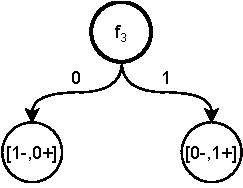
\includegraphics[scale = 0.9]{img/id7.pdf}
  \end{figure}
  Avendo per di più entrambi i risultati con distribuzione certa.\\
  Il nodo di $f_3$ sarà attaccato al nodo $[1-,1+]$ ``uscente'' da $f_2$,
  ottenendo così l'albero:
  \begin{figure}[H]
    \centering
    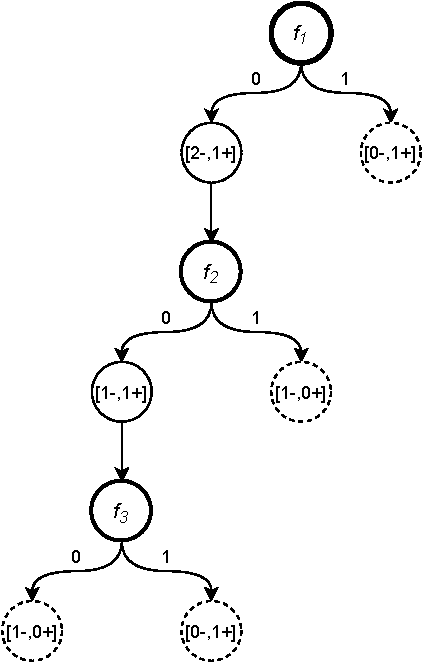
\includegraphics[scale = 1]{img/id8.pdf}
  \end{figure}
\end{esercizio}
\chapter{Reti neurali}
\section{Neurone biologico}
In natura l'operazione di \textit{learning} viene eseguita tramite il
\textbf{cervello}, che tramite i \textbf{neuroni}, delle cellule nervose, è in
grado di effettuare una miriade di operazioni in parallelo. Potenzialmente i
neuroni hanno un tempo di risposta nell'ordine dei millisecondi mentre in
circuito logico si aggira nell'ordine dei nanosecondi quindi la differenza deve
essere ricercata nell'\textit{architettura} del nostro cervello. La ``potenza di
calcolo'' del cervello è data dal funzionamento parallelo di $\sim 10^{11}$
neuroni, collegati tra loro da $\sim 10^5$ connessioni. Vediamo quindi
indicativamente gli elementi principali di un \textbf{neurone biologico}:
\begin{itemize}
  \item \textbf{corpo}, che implementa tutte le funzioni logiche del neurone
  \item \textbf{assone}, il canale di uscita verso gli altri neuroni, è quello
  che si occupa di trasmettere gli impulsi nervosi
  \item \textbf{dendrite}, la parte che permette al neurone di ricevere gli
  impulsi nervosi
  \item \textbf{sinapsi}, ovvero la regione funzionale in cui avviene lo scambio
  dei segnali, ovvero dove ogni singolo ramo terminale dell'assone
  (\textbf{bottone sinaptico}) del neurone (detto \textbf{neurone
    pre-sinaptico}) trasmette impulsi nervosi provenienti dal neurone ai
  dendriti di altri neuroni (detti \textbf{neuroni post-sinaptici})
\end{itemize}
Questa ``architettura'' è quindi basata sull'emissione di segnali da parte del
neurone. Questa azione dipende da vari fattori, come ad esempio la forza del
segnale ricevuto da altri neuroni e la forza delle connessioni di un neurone con
le sue sinapsi. Si ha che la \textbf{funzione di risposta} di un neurone è una
funzione non lineare impulso ricevuto dai dendriti. Dopo l'invio di un impulso
ogni neurone ha un tempo, detto \textbf{refractory time}, prima del quale poter
inviare un altro impulso. Si hanno infatti due stati possibili per il
\textit{neurone biologico}:
\begin{enumerate}
  \item \textbf{eccitazione}, quando il neurone invia, tramite le sinapsi,
  segnali (che per comodità computazionale chiamiamo già \textbf{pesati}) ai
  neuroni connessi
  \item \textbf{inibizione}, quando il neurone non invia segnali
\end{enumerate}
La \textbf{transizione di stato} dipende dall'entità complessiva dei segnali
eccitatori e inibitori ricevuti dal neurone.\\
Una legge importante è la \textbf{regola di Hebb} che indica che i cambiamenti
di forza delle connessioni delle sinapsi di due neuroni connessi è proporzionale
alla correlazione tra l'emissione di segnali dei neuroni stessi (ovvero se due
neuroni rispondono allo stesso input allora è bene che siano connessi).
\section{Neuroni formali}
Dopo una breve introduzione biologica possiamo alla definizione \textbf{formale
  e matematica} che verrà usato nello studio delle reti neurali. Questo modello
matematico è stato proposto da \textbf{McCulloch} e \textbf{Pitts} e definisce
formalmente un \textbf{neurone binario a soglia} come una quadrupla:
\[\langle n, C, W, \theta \rangle\]
dove:
\begin{itemize}
  \item $n$ specifica il \textbf{nome} del neurone stesso, una sorta di
  identificativo
  \item $C$ specifica l'\textbf{insieme degli input} $c_i$
  \item $W$ specifica il \textbf{vettore dei pesi} $w_i$, associati ad ogni
  input $c_i$. È una rappresentazione formale dei pesi delle sinapsi (e si nota
  che possono essere sia positivi che negativi)
  \item $\theta$ specifica la \textbf{soglia}, utile per definire quando un
  neurone manda effettivamente il segnale
\end{itemize}
Per definire i \textbf{due stati del neurone} si usa l'insieme $\{0,1\}$ o
l'insieme $\{-1,1\}$ (si ha infatti un \textbf{neurone binario}). La
\textbf{funzione di transizione} viene indicata con:
\[s(t+1)=1 \mbox{ \textnormal{sse} }\sum w_i\cdot s_i(t)\geq \theta\]
ovvero in un tempo successivo $t+1$ (con $s(t)$ che definisce uno stato al tempo
$t$) ho che il neurone emette il segnale (stato

pari ad 1) sse al tempo precedente $t$ ho avuto una somma pesata, tramite $w_i$,
degli input $c_i(t)$ maggiore della soglia
$\theta$.\\
L'insieme degli stati, rappresentato in modo binario, comporta che la funzione
di transizione sia una \textbf{funzione a scalino}:
\[f(x)=
  \begin{cases}
    1 &\mbox{ se } x\geq \theta\\
    0 &\mbox{ altrimenti}
  \end{cases}\,\,\,\mbox{   con }\,\,\, x=\sum w_i\cdot c_i
\]
\begin{figure}[H]
  \centering
  \psscalebox{1.0 1.0} % Change this value to rescale the drawing.
  {
    \begin{pspicture}(3,-0.965)(9.8,0.965)
      \psframe[linecolor=black, linewidth=0.04, dimen=outer]
      (4.0,0.71990234)(2.4,-0.8800976)
      \psline[linecolor=black, linewidth=0.04, arrowsize=0.05291667cm 2.0,
      arrowlength=1.4,arrowinset=0.0]{->}(0.8,0.71990234)(2.4,-0.08009765)
      \psline[linecolor=black, linewidth=0.04, arrowsize=0.05291667cm 2.0,
      arrowlength=1.4,arrowinset=0.0]{->}(0.8,-0.08009765)(2.4,-0.08009765)
      \psline[linecolor=black, linewidth=0.04, arrowsize=0.05291667cm 2.0,
      arrowlength=1.4,arrowinset=0.0]{->}(0.8,-0.8800976)(2.4,-0.08009765)
      \psline[linecolor=black, linewidth=0.04, arrowsize=0.05291667cm 2.0,
      arrowlength=1.4,arrowinset=0.0]{->}(4.0,-0.08009765)(5.6,-0.08009765)
      \psframe[linecolor=black, linewidth=0.04, dimen=outer]
      (7.2,0.71990234)(5.6,-0.8800976)
      \psline[linecolor=black, linewidth=0.04]
      (6.0,-0.48009765)(6.4,-0.48009765)(6.4,0.31990233)(6.8,0.31990233)
      \psline[linecolor=black, linewidth=0.04, arrowsize=0.05291667cm 2.0,
      arrowlength=1.4,arrowinset=0.0]{->}(7.2,-0.08009765)(8.4,-0.08009765)
      \rput[bl](3,-0.28009765){$\sum$}
      \rput[bl](6.5,-0.48009765){$\theta$}
      \rput[bl](8.4,-0.28009765){$\,output\mbox{ (esempio }\{0,1\}\mbox{)}$}
      \rput[bl](0.4,0.690990234){$c_1$}
      \rput[bl](0.4,-0.12009765){$c_2$}
      \rput[bl](0.4,-0.9300976){$c_n$}
      \rput[bl](0.4,-0.48009765){$\ldots$}
      \rput[bl](1.2,0.51990233){$w_1$}
      \rput[bl](1.2,-0.01990233){$w_2$}
      \rput[bl](1.2,-0.40009765){$w_n$}
      \rput[bl](4.0,-0.031990233){$\sum c_i\cdot w_i$}
    \end{pspicture}
  }
  \caption{Rappresentazione matematica del modello di McColluch e Pitts, ovvero
    rappresentazione della \textbf{Linear Treshold Unit (\textit{LTU})}}
  \label{fig:bin}
\end{figure}
Questo modello è comunque estremamente semplificato. L'insieme degli stati
potrebbe non essere booleano ma potrebbe essere $\mathbb{R}$, infatti anche
nella biologia il segnale in uscita dai neuroni è graduato e continuo. Si
potrebbe quindi avere una \textbf{funzione logistica o sigmoide}, dove, avendo
come insieme degli stati $\mathbb{R}$ si avrebbe:
\[f(x)=\frac{1}{1+e^{-x}}\,\,\,\,\mbox{   con } \,\,\,x=\sum w_i\cdot c_i\]
\section{Reti neurali artificiali}
Lo studio di un singolo neurone non è comunque particolarmente interessante. Si
introduce quindi lo studio di \textbf{reti neurali} dove vengono posti diversi
\textit{neuroni} in modo che possano fare qualcosa di utile.\\
Se dal singolo neurone voglio passare alla rete collego in modo orientato i
neuroni, di modo che l'output di uno sia l'input dell'altro. \\
Si hanno alcune \textbf{caratteristiche strutturali} delle \textit{reti neurali
  artificiali}:
\begin{itemize}
  \item hanno un gran numero di unità
  \item permettono operazioni elementari
  \item hanno un alto livello di interconnessione
\end{itemize}
Ci sono anche alcune \textbf{caratteristiche dinamiche}:
\begin{itemize}
  \item si hanno cambiamenti di stato in funzione dello stato dei neuroni
  collegati in input
  \item si ha una funzione di uscita per ogni unità
  \item si ha la modifica dello schema di connessione, tramite la modifica dei
  pesi, per l'apprendimento
\end{itemize}
Dal punto di vista formale, dovendo espandere le definizioni fatte nel caso del
singolo neurone a più neuroni, si lavora con:
\begin{itemize}
  \item una \textbf{matrice dei pesi} $W$, con i valori indicati tramite
  $w_{ij}$, per gli archi che collegano i neuroni. I pesi sono i \textit{pesi
    correnti} (un vettore di pesi per ogni neurone e quindi una matrice, che
  risulta a singolo colonna se ho un solo neurone)
  \item un \textbf{vettore delle soglie} $\Theta$, con i valori indicati tramite
  $\theta_i$, una per ogni neurone
  \item l'\textbf{input netto per il neurone $i$ al tempo $t$}, indicato con\\
  $n_i(t)=\sum_{j=1}^n w_{ij}\cdot s_j(t)-\theta_i$, quindi si ha che la soglia
  influisce già nell'input del neurone (e quindi non si può ragionare come se
  $\theta$ fosse un confronto a posteriori)
  \item la \textbf{funzione di transizione} indicata con $s_i(t+1)=g(n_i(t))$
\end{itemize}
L'output di un neurone è, a conti fatti, uno stato per un altro neurone.\\
Si hanno alcuni elementi caratterizzanti di una rete neurale:
\begin{itemize}
  \item il \textbf{tipo di unità}
  \item la \textbf{topologia}, ovvero la direzione delle connessioni
  (\textit{feedforward \textnormal{o} feedback}), il numero di neuroni (con più
  layer o solo uno, \textit{monostrato \textnormal{o} multistrato}) etc$\ldots$
  \item le \textbf{modalità di attivazione}, che può essere \textit{seriale
    ciclica, seriale probabilistica, parallela \textnormal{o} mista}
  \item un \textbf{algoritmo di apprendimento} con lo studio, in primis, dei
  pesi
\end{itemize}
\newpage
\subsection{Percettrone}
\begin{shaded}
  \textbf{Ripasso di algebra lineare}\\
  Per praticità ripasseremo i concetti fondamentali facendo riferimento a
  $\mathbb{R}^2$, formato quindi da elementi, dette coordinate, che sono coppie
  ordinate $(x_1,x_2)$ (rappresentabili con un punto nel piano o con un segmento
  orientato con partenza nell'origine e destinazione nelle coordinate del punto
  nel piano).\\
  Ricordiamo le operazioni fondamentali, dati $R$ pari a $(x_1,x_2)$ e $Q$ pari
  a $(x_3,x_4)$ 
  \begin{itemize}
    \item addizione: $P+Q=(x_1+x_3, x_2+x_4)$
    \item prodotto per uno scalare $\lambda\in\mathbb{R}$: $\lambda\cdot
    R=(\lambda\cdot x_1,\lambda\cdot x_2)$
    \item prodotto scalare tra vettori: $\langle P,Q\rangle\equiv P\cdot Q^T =
    \sum_{i=1}^n r_i\cdot q_i$ 
    (dove $r_i$ e $q_i$ sono rispettivamente gli elementi di $R$ e $Q$
    all'indice $i$)
  \end{itemize}
  Ricordiamo la \textit{norma} di un vettore $X$:
  \[\norm{X}=\equiv\sqrt{X\cdot X^T}=\sqrt{\sum_{i=1}^n x_i\cdot
      x_i}=\sqrt{\langle X,X\rangle}\] 
  Con $X=0$ indichiamo il \textit{vettore nullo} (che ha anche norma nulla).\\
  Definiamo il \textit{versore} (\textit{vettore unitario}) come:
  \[\frac{X}{\norm{X}},\,\,\,X\neq 0\]
  In $\mathbb{R}^2$ l'angolo $\theta$ sotteso tra due vettori $X$ e $Y$ è:
  \[\cos\theta=\frac{\langle X,Y\rangle}{\norm{X}\cdot \norm{Y}}\]
  La proiezione di un vettore $X$ sul vettore $Y$ è:
  \[X_Y=\norm{X}\cdot \cos\theta\]
  Si hanno quindi tre casi:
  \begin{enumerate}
    \item $\theta < 90 \iff \langle X,Y\rangle >0$
    \item $\theta > 90 \iff \langle X,Y\rangle <0$
    \item $\theta = 90 \iff \langle X,Y\rangle =0$
  \end{enumerate}
  (quindi disegnando una retta sul piano tutti i punti sopra di essa
  apparterranno ad una certa classe e quelli sotto ad un'altra).\\
  Posso definire una retta $r$ che passa per l'origine in  $\mathbb{R}^2$
  assegnando un vettore $W=(w_1,w_2)$ ad essa ortogonale, infatti tutti i punti,
  ovvero vettori, $X=(x_1,x_2)$ sulla retta sono ortogonali a $W$:
  \[\langle W,X\rangle=w_1\cdot x_1+w_2\cdot x_2=0 \]
  Quindi la retta (ovvero l'iperpiano) mi separa due semispazi, a seconda che
  $\langle X,W\rangle$ sia strettamente positivo o strettamente negativo.\\
  Generalizzando ora a $n$ dimensioni ho che, dato l'iperpiano $h$ (di
  dimensione $n-1$):
  \begin{itemize}
    \item se $h$ passa dall'origine allora si ha l'equazione $\langle X,Y\rangle
    =0$
    \item se non passa per l'origine $\langle X,Y\rangle +b=0$ 
    
  \end{itemize}
  I vettori in un iperpiano si proiettano tutti nello stesso modo e i punti ad
  un lato e all'altro dell'iperpiano sono distinti dal fatto che $\langle
  X,Y\rangle +b$ sia strettamente positiva o strettamente negativa
\end{shaded}
Il percettrone è la tipologia di rete neurale più semplice, sono infatti una
semplificazione estrema del sistema nervoso.
\begin{definizione}
  Un percettrone è una collezione di neuroni, di cardinalità $M$, a cui viene
  aggiunto un insieme di nodi in input, di cardinalità $N$ (generalmente
  diversa da quella della collezione di neuroni). Generalmente gli input sono
  pesati e con la notazione $w_{ij}$ indichiamo il peso della connessione tra il
  nodo $i$-simo in input e il neurone $j$-simo.\\
  I neuroni sono tra loro completamente indipendenti comportando anche un
  insieme di elementi in output. Nel caso semplice di funzioni di transizione
  binarie l'output sarà quindi un vettore binario contenente all'indice $k$-simo
  1 se il neurone $k$ ha inviato il segnale o 0 altrimenti. \\
  Solitamente coi percettroni si parla di \textit{learning supervisionato}.
\end{definizione}
Dal punto di vista geometrico il vettore dei pesi $W$ rappresenta un
\textbf{iperpiano} (che è una retta in $\mathbb{R}^2$) che separa i possibili
vettori di input in due classi, a seconda che formino con $W$ un angolo acuto o
ottuso. \\
Studiamo quindi l'apprendimento del percettrone.\\
Come abbiamo visto l'output è rappresentato da un vettore booleano
rappresentante 1 in posizione $k$ in corrispondenza del neurone $k$-simo che ha
inviato il segnale o 0 altrimenti. A questo risultato si giunge tramite un certo
input pesato e, essendo un training supervisionato, esso viene
verificato. Qualora un risultato non vada bene bisogna procedere cambiando i
pesi. Il problema è appunto la scelta dei pesi, che non sono conoscibili a
priori. Un peso troppo alto porta un neurone a mandare il segnale anche quando
non dovrebbe mentre un peso troppo basso impedisce l'invio del segnale anche
quando il neurone dovrebbe. Preso un neurone $k$ che porta un risultato errato
posso definire una \textbf{function error} come:
\[E=y_k-t_k\]
dove:
\begin{itemize}
  \item $y_k$ è l'output del neurone
  \item $t_k$ è il target atteso per quel neurone
\end{itemize}
Per tale neurone bisognerà sistemare tutti i pesi $w_{ik}$.\\
Se $E$ è negativa allora il neurone avrebbe dovuto emettere il segnale ma non lo
ha fatto e quindi bisogna aumentare il peso e viceversa (nel caso binario o ho
-1 o 1). Bisogna però considerare che l'input potrebbe essere negativo e quindi
anche in pesi devono poter essere negativi. Perfezioniamo quindi il conto della
differenza di peso necessaria con la moltiplicazione di $E$ (messa in negativo
in modo da eventualmente ``sistemare'' il segno per input negativi) per l'input:
\[\Delta w_{ik}=-(y_k-t_k)\times c_i\]
In questo discorso bisogna inserire anche la soglia, importante per input
specifici (basti pensare ad un input pari a 0 che annullerebbe ogni cambio di
peso secondo la formula precedente). Per ora trascureremo tali casi anche se una
semplice soluzione per un caso limite come quello di avere solo input nulli, è
quella di aggiungere un \textbf{nodo bias}, di valore $-1$, collegato ai neuroni
con peso nullo.\\
Viene anche introdotto il \textbf{learning rate (\textit{tasso di
    apprendimento})} $\eta$, utile per stabilire la velocità di apprendimento
della rete. Si ottiene quindi:
\[w_{ij}\gets w_{ij}-\eta\cdot(y_j-t_j)\times c_i\]
In pratica $\eta$ decide quanto cambiare il peso (e se si vuole trascurare il
parametro basta porre $\eta =1$). L'uso di tale parametro migliora la stabilità
della \textit{rete neurale} che non avrà cambi di peso eccessivi, anche se
questo comporta tempi di apprendimento più estesi. Tipicamente si ha che:
\[0.1\leq\eta\leq 0.4\]
Si ha che ad ogni iterazione ci si aspetta un miglioramento della
\textit{rete neurale} (e questo miglioramento è dimostrabile). Viene imposto
quindi un limite $T$ di iterazioni entro le 
quali interrompere l'apprendimento anche se non si è arrivati al risultato
corretto.\\
Vediamo due teoremi utili per lo studio dell'apprendimento del percettrone su
due classi $A$ e $B$, banalmente rappresentanti, nella nostra situazione binaria
e semplificata, il caso in cui si abbia il
neurone che emette il segnale (valore 1 in output) o altrimenti (valore 0 in
output). Nel nostro caso le classi sono discriminabili.
\begin{teorema}[Teorema di convergenza]
  Comunque si scelgano i pesi iniziali, se le classi A e B sono discriminabili,
  la procedura di apprendimento termina dopo un numero finito di passi
\end{teorema}
\begin{teorema}[Teorema di Minsky e Papert]
  La classe delle forme discriminabili da un percettrone semplice è
  limitata alle forme linearmente separabili
\end{teorema}
In base a questo si distinguerà in:
\begin{itemize}
  \item \textbf{addestramento separabile}, quando si ha un iperpiano che separa
  le istanze positive e negative
  \item \textbf{addestramento non separabile}
\end{itemize}
Per capire il discorso della \textbf{separabilità} vediamo un esempio.
\begin{esempio}
  Vediamo un esempio che tratta l'addizione binaria, ovvero l'\textit{or
    esclusivo}.
  Le possibili istanze sono rappresentate nel piano:
  \begin{figure}[H]
    \centering
    \psscalebox{1.0 1.0} % Change this value to rescale the drawing.
    {
      \begin{pspicture}(0,-1.9534792)(5.906958,1.9534792)
        \psline[linecolor=black, linewidth=0.04,
        arrowsize=0.05291667cm 2.0,arrowlength=1.4
        ,arrowinset=0.0]{->}(2.4,-1.9534792)(2.4,1.6465209)(2.4,2.046521)
        \psline[linecolor=black, linewidth=0.04,
        arrowsize=0.05291667cm 2.0,arrowlength=1.4,
        arrowinset=0.0]{->}(1.6,-1.1534791)(6.0,-1.1534791)
        \psdots[linecolor=black, dotsize=0.4](2.4,0.84652084)
        \psdots[linecolor=black, dotsize=0.4](4.4,0.84652084)
        \psdots[linecolor=black, dotsize=0.4](4.4,-1.1534791)
        \psdots[linecolor=black, dotsize=0.4](2.4,-1.1534791)
        \rput[bl](0.4,0.68652084){$0\oplus 1=1$}
        \rput[bl](0.4,-0.7534792){$0\oplus  1=0$}
        \rput[bl](3.4,-0.7534792){$1\oplus 0=1$}
        \rput[bl](3.4,1.2465209){$1\oplus 1=0$}
      \end{pspicture}
    }
  \end{figure}
  Ho quindi che nessuna retta potrà separare tutti i punti e
  quindi i punti a valore 1 \textbf{non sono linearmente separabili} da quelli a
  valore 0.\\
  Si vorrebbe cercare un neurone binario a soglia tale che:
  \[x\oplus y=1\iff \alpha\cdot x+\beta\cdot y\geq \lambda\]
  Tale neurone si rappresenterebbe con:
  \begin{figure}[H] 
    \centering
    \psscalebox{1.0 1.0} % Change this value to rescale the drawing.
    {
      \begin{pspicture}(0,-1.9534792)(5.906958,1.9534792)
        \pscircle[linecolor=black, linewidth=0.04,
        dimen=outer](3.2,0.24245118){0.8}
        \psline[linecolor=black, linewidth=0.04,
        arrowsize=0.05291667cm 2.0,arrowlength=1.4,
        arrowinset=0.0]{->}(0.4,0.64245117)(2.4,0.64245117)
        \psline[linecolor=black, linewidth=0.04, arrowsize=0.05291667cm 2.0,
        arrowlength=1.4,arrowinset=0.0]{->}(0.4,-0.15754883)(2.4,-0.15754883)
        \psline[linecolor=black, linewidth=0.04, arrowsize=0.05291667cm 2.0,
        arrowlength=1.4,arrowinset=0.0]{->}(4.0,0.24245118)(6.0,0.24245118)
        \rput[bl](0.0,0.56245117){$x$}
        \rput[bl](0.0,-0.32754883){$y$}
        \rput[bl](1.2,0.8245117){$\alpha$}
        \rput[bl](1.2,0.024245118){$\beta$}
        \rput[bl](3.07,0.115754886){$\lambda$}
        \rput[bl](6.2,0.0824245118){$x\oplus y$}
      \end{pspicture}
    }
  \end{figure}
  ma appunto tale neurone non può esistere in quanto non potrei mai separare
  i punti a valori 1 e quelli a valore 0 con una retta. Posso infatti separare o
  singoli punti o coppie di punti a valore opposto o triple di punti ma non
  potrò mai avere separati insiemi con tutti gli 0 e tutti gli 1.
\end{esempio}
\begin{teorema}
  Se l'insieme degli input estesi è partito in due classi linearmente separabili
  allora:
  \[\exists\,\,W\mbox{ t.c }
    \begin{cases}
      1 &\mbox{ se } \sum w_i\cdot c_i \geq 0\\
      0 &\mbox{ se } \sum w_i\cdot c_i < 0
    \end{cases}
  \]
  con $W$ \textbf{vettore dei pesi}.
\end{teorema}
Vediamo quindi l'algoritmo di learning per un percettrone, data la
\textbf{funzione di transizione} per un input di cardinalità $m$ e $n$ neuroni:
\[
  y_j=g\left(\sum_{i=0}^m w_{ij}\cdot c_i \right)=
  \begin{cases}
    1 &\mbox{ se } \sum_{i=0}^m w_{ij}\cdot c_i > 0\\
    0 &\mbox{ se } \sum_{i=0}^m w_{ij}\cdot c_i \leq 0
  \end{cases}
\]
Vediamo quindi l'algoritmo di apprendimento del percettrone:
\begin{algorithm}[H]
  \begin{algorithmic}
    \Function{perceptron-learning}{}
    \State \textit{\color{gray}{\# Inizializzazione}}
    \State \textit{si imposta tutti i pesi $w_{ij}$ a valori casuali piccoli
    (anche negativi)}
    \State \textit{\color{gray}{\# Training}}
    \For {\textit{$T$ iterazioni \textbf{o} fino a che tutti gli output non sono
    corretti}}
    \For {\textit{ogni vettore input}}
    \State \small{\color{gray}{\textit{\# calcolo l'attivazione di ogni neurone
    $j$ }}}
    \State \small{\color{gray}{\textit{\# tramite la funzione di transizione
    $g$:}}} 
    \State $y_j=g\left(\sum_{i=0}^m w_{ij}\cdot c_i \right)=
    \begin{cases} 1
      &\mbox{ se } \sum_{i=0}^m w_{ij}\cdot c_i > 0\\ 0 &\mbox{ se }
      \sum_{i=0}^m w_{ij}\cdot c_i \leq 0
    \end{cases}$ 
    \State {\textit{\color{gray}\# aggiorno ogni peso individualmente}}
    \State {\textit{\color{gray}\# nella prossima iterazione avrò nuovi pesi}}
    \State $w_{ij}\gets w_{ij}-\eta\cdot(y_j-t_j)\times c_i$
    \EndFor
    \EndFor
    \State {\textit{\color{gray}\# Recall}}
    \State \small{\color{gray}{\textit{\# ricalcolo l'attivazione di ogni
    neurone $j$ tramite:}}} 
    \State $y_j=g\left(\sum_{i=0}^m w_{ij}\cdot c_i \right)=
    \begin{cases} 1
      &\mbox{ se } w_{ij}\cdot c_i > 0\\ 0 &\mbox{ se }
      w_{ij}\cdot c_i \leq 0
    \end{cases}$
    \EndFunction
  \end{algorithmic}
  \caption{Algoritmo di learning del percettrone}
\end{algorithm}
La complessità dell'algoritmo è $O(Tnm)$.\\
Si può dimostrare, tramite il \textbf{teorema della convergenza del percettrone}
che dopo $\beta$ modifiche di peso il percettrone classifica 
correttamente ogni input anche se tale $\beta$ non è il reale numero di stadi e
dipende dall'output.\\
L'algoritmo di apprendimento del percettrone quindi \textit{converge} alla
classificazione corretta quindi se:
\begin{itemize}
  \item i dati di training sono linearmente separabili
  \item $\eta$ è abbastanza piccolo
\end{itemize}
\subsubsection{Teorema di convergenza del percettrone}
\textbf{Per completezza vengono aggiunte le note finali sul teorema presenti
  nelle slide}.
\begin{teorema}
  Se l'insieme degli input estesi è partito in due classi linearmente separabili
  $A$ e $B$ allora é possibile trovare un vettore di pesi $w$ tale che:
  \[
    \begin{cases}
      \langle w, x\rangle\geq 0&\mbox{ se }x\in A\\
      \langle w, x\rangle < 0&\mbox{ se }x\in B
    \end{cases}
  \]
  Quindi:
  \begin{itemize}
    \item si parte con $w$ arbitrario
    \item si classifica un punto $x$:
    \begin{itemize}
      \item se la risposta è corretta si ha $w'\gets w$
      \item se la risposta è errata:
      \[
        \begin{cases}
          w'\gets w+x&\mbox{ se }x\in A\\
          w'\gets w-x&\mbox{ se }x\in B\\
        \end{cases}
      \]
    \end{itemize}
  \end{itemize}

\end{teorema}
\begin{proof}
  Vediamo la prova della correttezza del teorema.\\
  Se si ha $x\in A$ allora si ha $\langle w, x\rangle<0$ infatti, poiché:
  \[\langle x, x\rangle\geq 0\]
  si ha che:
  \[\langle w', x\rangle=\langle (w+x), x\rangle=\langle w, x\rangle+\langle x,
    x\rangle>\langle w, x\rangle\]
  Quindi $w'$ classifica $x$ in modo più corretto di $w$ anche se altri input
  possono essere classificati "meno correttamente".
\end{proof}
\begin{proof}
  Passiamo ora alla convergenza.\\
  Consideriamo quindi $A'=A\cup B'$ con:
  \[B'=\{-x|\,x\in B\}\]
  e cerchiamo un $v$ tale che:
  \[\langle v, x\rangle\geq 0,\,\,\forall\,x\in A'\]
  Si hanno quindi:
  \begin{itemize}
    \item la \textbf{sequenza di addestramento} $\{x_i\}_{i\in N}$ dove $x_i\in
    A'$ e quindi la sequenza ontiene infiniti elementi sia di $A$ che di $B'$
    \item la \textbf{sequenza di pesi} $\{w_i\}_{i\in N}$ dove si parte
    arbitrariamente con $w_0=0$ e si procede con:
    \[
      \begin{cases}
        w_{k+1}\gets w_k &\mbox{ se }\langle w_k, x_k\rangle\geq 0\\
        w_{k+1}\gets w_k+x_k&\mbox{ altrimenti}
      \end{cases}
    \]
  \end{itemize}
  Si hanno quindi:
  \begin{itemize}
    \item la \textbf{sequenza di pesi modificata} $\{v_i\}_{i\in N}$ 
    \item la \textbf{sottosequenza di training corrispondente} $\{v_i\}_{i\in N}$ 
  \end{itemize}
  Di modo che le coppie $(v_i,t_i)$ corrispondano ai $w_j$ tali per cui $w_j\neq
  w_{j+1}$.\\
  Ad esempio per:
  \[w_0\neq w_1=w_2=w_3\neq w_4=w_5=w_6\neq w_7\neq w_8\cdots\]
  avremo:
  \begin{itemize}
    \item $(v_0,t_0)$ associati a $w_0$
    \item $(v_1,t_1)$ associati a $w_3$
    \item $(v_2,t_2)$ associati a $w_6$
    \item $(v_3,t_3)$ associati a $w_7$
  \end{itemize}
  Avendo:
  \[\langle v_i,t_i\rangle<0\,\,\,\forall i\]
  e avendo:
  \[v_{i+1}=v_i+t_i=v_{i-1}+t_{i-1}+y_i=\sum_{k=0}^i t_i\]
  e quindi la sequenza $\{v_i\}$ è \textbf{finita}.
\end{proof}
\begin{proof}
  Uniamo matematicamente in una sola dimostrazione.\\
  Sia $w$ una qualsiasi soluzioni che sappiamo esistere per ipotesi. Si ha che:
  \[\langle v, x\rangle\geq 0,\,\,\forall\,x\in A'\]
  Pongo quindi:
  \[\alpha=\min(\langle x,w\rangle,\,\,\forall\,x\in A')\]
  sapendo che:
  \[v_{i+1}=v_i+t_i=v_{i-1}+t_{i-1}+y_i=\sum_{k=0}^it_i\]
  ho che:
  \[\langle v_{i+1},w\rangle=\langle \left(\sum_{k=0}^i t_k \right),
    w\rangle\geq (i+1)\cdot\alpha\]
  ma usando il teorema di \textbf{Cauchy-Schwarz} si ha che:
  \[(\langle v_{i+1},w\rangle)^2\leq \langle |v_{i+1}|^2,|w|^2\rangle\]
  ottenendo che:
  \[|v_{i+1}|^2\geq \frac{(i+1)^2\cdot \alpha^2}{|w|^2}\]
  Pongo quindi:
  \[M=\max\{|x|^2|,\,x\in A'\}\]
  si ha che, avendo $\langle v_{1},t_i\rangle<0$:
  \[|v_{i+1}|^2=|v_i+t_i|^2=|v_i|^2+2\cdot\langle v_{i},t_i\rangle+|t_i|^2\leq
    |v_i|^2+|t_i|^2\]
  Si ha, di conseguenza:
  \[|v_{i+1}|^2\leq \sum_{k=1}^i |t_i|^2\leq i\cdot M\]
  Unendo quest'ultima con $|v_{i+1}|^2\geq \frac{(i+1)^2\cdot \alpha^2}{|w|^2}$
  si ha che:
  \[f(i)=\frac{j^2\cdot \alpha^2}{|w|^2}\leq |v_{i+1}|^2\leq i\cdot M=g(i)\]
  avendo che $\frac{j^2\cdot \alpha^2}{|w|^2}$ è quadratico in $i$ e $ i\cdot M$
  lineare in $i$.\\
  Si ottiene quindi che:
  \[i\leq\frac{M\cdot |w|^2}{\alpha^2}=\beta\]
  Quindi dopo $\beta$ modifiche di peso il percettrone classifica correttamente
  ogni input.
\end{proof}





\subsection{Discesa lungo il gradiente}
\textbf{Le formule più complesse sono solo di bellezza.}\\
\noindent
Fino ad ora il singolo neurone rappresentava un singolo iperpiano che veniva
``spostato'' per dividere le istanze positive e quelle negative.\\
Ora introduciamo che ad ogni passo di aggiornamento si aggiornano i pesi e se,
mano a mano che cambio i pesi, misuro l'errore sul dataset del mio sistema. Si
può quindi far ``scendere'' questo errore e ci si augura che ci sia una costante
di discesa dell'errore. L'errore complessivo sul dataset $D$ è calcolato come:
\[E[w_0,\ldots, w_n]=\frac{1}{2}\sum_{d\in D}(t_d-y_d)^2\]
Si calcola il gradiente della curva degli errori e si punta ad essere sempre in
``discesa'' lungo la curva dell'errore, aggiustando in modo opportuno i pesi.\\
La strategia di apprendimento sarà quella di minimizzare una opportuna
funzione dei pesi $w_i$. Mi devo spostare verso un punto di minimo, scendendo
nel grafico della funzione costruita tra pesi ed errore complessivo (quindi
anche in più dimensioni).\\
A livello di conti si ha che:
\[\nabla E[w]=\left[\frac{\partial E}{\partial w_0},\ldots,\frac{\partial
      E}{\partial w_n}\right]\]
e quindi aggiornando i pesi come:
\[w'=w+\delta w= w-\eta\nabla E[w]\]
Si ha quindi:
\[\Delta w_i=-\eta\frac{\partial E}{\partial w_i}=-\eta\frac{\partial}{\partial
    w_i}\cdot \frac{1}{2}\sum_d (t_d-y_d)^2\]
\[=-\eta\frac{\partial}{\partial
    w_i}\cdot \frac{1}{2}\sum_d (t_d-\sum_i w_i\cdot x_{di})^2=
  -\eta\sum_d(t_d-y_d)\cdot(-x_i)\]
Si vuole addestrare quindi cambiando costantemente la sequenza di pesi del
vettore di input $\langle( x_1, \ldots x_n),t\rangle$, con $t$ output
corrispondente.\\
$w_i$ è inizializzato con un valore piccolo e si ha l'algoritmo:
\begin{algorithm}[H]
  \begin{algorithmic}
    \Function{grad}{}
    \State \textit{inizializzo ogni $\Delta w_i$ a $0$}
    \For {\textit{ogni input $\langle( x_1, \ldots x_n),t\rangle$}}
    \State \textit{invio l'input $( x_1, \ldots x_n)$ all'unità lineare e
    calcola l'output $y$} 
    \State \textit{aggiorno la variazione dei pesi:}
    \[\Delta w_i=\Delta w_i+\eta\cdot (t-y)\cdot x_i\]
    \EndFor
    \State \textit{aggiorno i pesi:}
    \[w_i=w_i+\Delta w_i\]
    \EndFunction
  \end{algorithmic}
  \caption{Algoritmo di discesa lungo il gradiente}
\end{algorithm}
Abbiamo una \textbf{modalità Batch}, quindi computazionalmente costosa:
\[w=w-\eta\cdot\nabla E_D[W]\]
Si può avere una \textbf{modalità incrementale}:
\[w=w-\eta\cdot\nabla E_d[W]\]
calcolata sui singoli esempi $d$:
\[E_d[w]=\frac{1}{2}(t_d-y_d)^2\]
La discesa lungo il gradiente incrementale può approssimare la discesa lungo
il gradiente Batch arbitrariamente se $\eta$ è abbastanza piccolo.\\
Rispetto a quanto visto per il percettrone la discesa lungo il gradiente
converge all'ipotesi con il minimo errore quadratico se  $\eta$ è abbastanza
basso, anche per dati di training molto rumorosi.
\subsection{Reti multistrato}
\textbf{Le formule più complesse sono solo di bellezza.}\\
\noindent
Passiamo quindi dal percettrone ad una rete a due strati, cambiando quindi la
gestione dei pesi.\\
Devo avere sempre un gradiente dei pesi, che ora avranno doppio indice per
indicare anche l'unità di riferimento, che scende:
\[\frac{\partial E}{\partial w_{ij}}=\frac{\partial E}{\partial y_{j}}\cdot
  \frac{\partial y_j}{\partial w_{ij}}=-(t_j-y_j)\cdot \frac{\partial
    y_j}{\partial w_{ij}}=-\delta_j\cdot\frac{\partial \sum_i w_{ij}\cdot
    x_j}{\partial w_{ij}}=-\delta_j\cdot x_i\]
Si ha quindi:
\[\Delta w_{ij}=\eta\cdot \delta_j\cdot x_i\]
detta \textbf{regola delta}, che è l'evoluzione di quanto detto per il
percettrone in merito alla variazione dei pesi.\\
Si ha che la convergenza a un minimo globale é garantita per funzioni di
attivazione lineari senza unità nascoste e per dati consistenti.\\
Si introduce una nuova funzione di attivazione, detta \textbf{sigmoide}, che
comporta l'\textbf{unità sigmoide}. La funzione sigmoide è:
\[y=\sigma(net)=\frac{1}{1+e^{-net}}\]
Tale funzione è derivabile, infatti:
\[\dd \sigma(x)=\sigma(x)\cdot (1-\sigma(x))\]
riprendendo la figura \ref{fig:bin} si ha quindi in primis l'aggiunta del nodo
bias e poi il cambio della funzione a scalino con il \textbf{sigmoide}. L'output
invece non sarà più binario ma un certo $y$.\\
Si hanno quindi in primis le \textbf{reti multistrato feedforward} con le
seguenti caratteristiche:
\begin{itemize}
  \item si hanno strati intermedi tra input e output
  \item si hanno connessioni da strati di livello basso a strati di livello
  alto, solitamente mono direzionali
  \item non si hanno all'interno di uno stesso strato
  \item il neurone ha uno stato booleano $x\in\{0,1\}$
  \item si ha la seguente funzione di transizione:
  \[x_k=\sigma\left(\sum_{j}w_{jk}\cdot x_j\right)\]
  con $x_j$ che può essere in alcuni
  casi un input istanza e in altri lo stato di altri neuroni, a seconda
  dell'altezza del livello in cui mi trovo
  \item per ogni configurazione $x$ del primo strato (ingresso), la rete calcola
  una configurazione $y$ dell'ultimo strato (uscita). Normalmente avremo uno
  strato nascosto più grande (poco) di quello d'uscita (anche se non si ha una
  regola per dimensionare lo strato nascosto). Raramente useremo più strati
  nascosti
\end{itemize}
\begin{figure}
  \centering
  \psscalebox{0.8 0.8} % Change this value to rescale the drawing.
  {
    \begin{pspicture}(-3,-4.18)(7.52,4.18)
      \definecolor{colour2}{rgb}{0.96862745,0.3019608,0.3019608}
      \definecolor{colour1}{rgb}{0.003921569,0.003921569,0.003921569}
      \definecolor{colour3}{rgb}{0.039215688,0.5647059,0.1882353}
      \definecolor{colour4}{rgb}{0.078431375,0.28627452,0.8784314}
      \pscircle[linecolor=black, linewidth=0.04, dimen=outer]
      (2.4,2.7049024){0.4}
      \pscircle[linecolor=black, linewidth=0.04, dimen=outer]
      (2.4,0.70490235){0.4}
      \pscircle[linecolor=black, linewidth=0.04, dimen=outer]
      (4.0,0.70490235){0.4}
      \pscircle[linecolor=black, linewidth=0.04, dimen=outer]
      (0.8,0.70490235){0.4}
      \pscircle[linecolor=black, linewidth=0.04, dimen=outer]
      (2.4,-0.8950977){0.4}
      \pscircle[linecolor=black, linewidth=0.04, dimen=outer]
      (4.0,-0.8950977){0.4}
      \pscircle[linecolor=black, linewidth=0.04, dimen=outer]
      (0.8,-0.8950977){0.4}
      \pscircle[linecolor=black, linewidth=0.04, dimen=outer]
      (1.6,-2.8950977){0.4}
      \pscircle[linecolor=black, linewidth=0.04, dimen=outer]
      (3.2,-2.8950977){0.4}
      \psline[linecolor=black, linewidth=0.04, arrowsize=0.05291667cm 2.0,
      arrowlength=1.4,arrowinset=0.0]{<-}(2.4,2.3049023)(0.8,1.1049024)
      \psline[linecolor=black, linewidth=0.04, arrowsize=0.05291667cm 2.0,
      arrowlength=1.4,arrowinset=0.0]{<-}(2.4,2.3049023)(2.4,1.1049024)
      \psline[linecolor=black, linewidth=0.04, arrowsize=0.05291667cm 2.0,
      arrowlength=1.4,arrowinset=0.0]{<-}(2.4,2.3049023)(4.0,1.1049024)
      \psline[linecolor=black, linewidth=0.04, arrowsize=0.05291667cm 2.0,
      arrowlength=1.4,arrowinset=0.0]{<-}(0.8,-1.2950977)(1.6,-2.4950976)
      \psline[linecolor=black, linewidth=0.04, arrowsize=0.05291667cm 2.0,
      arrowlength=1.4,arrowinset=0.0]{<-}(0.8,-1.2950977)(3.2,-2.4950976)
      \psline[linecolor=black, linewidth=0.04, arrowsize=0.05291667cm 2.0,
      arrowlength=1.4,arrowinset=0.0]{<-}(2.4,-1.2950977)(1.6,-2.4950976)
      \psline[linecolor=black, linewidth=0.04, arrowsize=0.05291667cm 2.0,
      arrowlength=1.4,arrowinset=0.0]{<-}(2.4,-1.2950977)(3.2,-2.4950976)
      \psline[linecolor=black, linewidth=0.04, arrowsize=0.05291667cm 2.0,
      arrowlength=1.4,arrowinset=0.0]{<-}(4.0,-1.2950977)(3.2,-2.4950976)
      \psline[linecolor=black, linewidth=0.04, arrowsize=0.05291667cm 2.0,
      arrowlength=1.4,arrowinset=0.0]{<-}(4.0,-1.2950977)(1.6,-2.4950976)
      \psdots[linecolor=black, dotsize=0.04](1.2,-0.09509765)
      \psdots[linecolor=black, dotsize=0.04](1.6,-0.09509765)
      \psdots[linecolor=black, dotsize=0.04](2.0,-0.09509765)
      \psdots[linecolor=black, dotsize=0.04](2.8,-0.09509765)
      \psdots[linecolor=black, dotsize=0.04](3.2,-0.09509765)
      \psdots[linecolor=black, dotsize=0.04](3.6,-0.09509765)
      \psframe[linecolor=colour2, linewidth=0.04, dimen=outer]
      (4.4,-2.0950975)(0.4,-3.6950977)
      \rput[bl](1.2,-4.0950975){\textcolor{colour1}{strato di input}}
      \rput[bl](1,3.6049025){\textcolor{colour1}{strato di output}}
      \rput[bl](5,-0.19509765){\textcolor{colour1}{strati nascosti}}
      \psframe[linecolor=colour3, linewidth=0.04, dimen=outer]
      (4.0,3.5049024)(0.8,1.9049023)
      \psframe[linecolor=colour4, linewidth=0.04, dimen=outer]
      (4.8,1.5049024)(0.0,-1.6950977)
    \end{pspicture}
  }
  \caption{Rappresentazione stilizzata di rete multistrato}
\end{figure}
Quindi fissata una mappa $f$ tra input e output, sulla base degli stimoli $x_i$,
la rete cambia i pesi in modo che dopo un numero di passi $s$ si abbia l'output
$y_k$ tale che $f(x_k)=y_k,\forall\,k>s$ (almeno approssimativamente). Per la
modifica bisogna minimizzare un c\textbf{riterio di discrepanza} tra risposta
della rete e risposta desiderata.\\
In questo modo potremmo anche risolvere il problema dell'\textit{or esclusivo},
aggiungendo uno strato nascosto.\\
Viene aumentata la potenza rispetto al percettrone, permettendo una
classificazione \textbf{altamente non lineare}.\\
Si hanno quindi $u_1,\ldots, u_n$ neuroni divisi in:
\begin{itemize}
  \item unità di input
  \item unità nascoste
  \item unità di output
\end{itemize}
Si hanno inoltre:
\begin{itemize}
  \item pesi $w_jj$ per ogni coppia che voglio connettere
  \item stati di attivazione $s_j\in \mathbb{R}$
  \item input netto a $u_j$: $n_i=\sum_{i=0}^n w_{ij}\cdot s_i$
  \item funzione di transizione sigmoide:
  \[s_j(t+1)=\frac{1}{1+e^{-n_i(t)}}\]
\end{itemize}
Lo stato di uscita è determinato da una serie di strati profondi. Dato un input
$x$, un output target $t$ e un output effettivo $y$ abbiamo la solita forma
quadratica:
\[E=\frac{1}{2}\sum_j(t_j-y_j)^2\]
che dipende anche dagli strati nascosti. In ogni caso si ha:
\[\Delta w_{ij}=-\eta\cdot\frac{\partial E}{\partial w_{ij}}\]
poiché:
\[\frac{\partial E}{\partial w_{ij}}= \frac{\partial E}{\partial n_{j}}\cdot
  \frac{\partial n_j}{\partial w_{ij}}= \frac{\partial E}{\partial n_{j}}\cdot
  s_j=(def)-\delta_j\cdot s_j\]
e si cerca:
\[\delta_j=-\frac{\partial E}{\partial n_{j}}\]
Abbiamo quindi l'\textbf{algoritmo di retropropagazione} che si divide in 5
passi:
\begin{enumerate}
  \item \textbf{input}: al neurone di input $u_j$ viene assegnato lo stato $x_j$
  
  \item \textbf{propagazione}: si calcola lo stato dei neuroni nascosti o di
  output $u_j$:
  \[s_j=f_j(n_j)\]
  \item \textbf{confronto}: per ogni neurone di output $u_j$, noto l’output
  atteso $t_j$, si calcola:
  \[\delta_j=f_j(n_j)\cdot(t_j-y_j))\]
  \item \textbf{retropropagazione dell’errore}: per ogni neurone nascosto $u_j$,
  si calcola:
  \[\delta_j=f_j(n_j)\cdot\left(\sum_h w_{ih}\cdot \delta_h\right)\]
  \item \textbf{aggiornamento dei pesi}: si ha:
  \[w_{ij}=w_{ij}+\eta\cdot \delta_i\cdot s_j\]
\end{enumerate}
Vediamo quindi l'algoritmo:
\begin{algorithm}[H]
  \begin{algorithmic}
    \Function{ret-prog}{}
    \State \textit{inizializzo ogni $\Delta w_i$ ad un valore piccolo casuale}
    \While {\textit{non raggiungimento della condizione di terminazione}}
    \For {\textit{ogni esempio $\langle (x_1,\ldots, x_n),t\rangle$}}
    \State \textit{immetto l'input $( x_1, \ldots x_n)$ nella rete e calcolo
    $y_k$}  
    \For {\textit{ogni unità di output $k$}}
    \[\delta_k=y_k\cdot(1-y_k)\cdot(t_k-y_k)\]
    \EndFor
    \For {\textit{ogni unità nascosta $h$}}
    \[\delta_h=y_h\cdot(1-y_h)\cdot\sum_k w_{hk}\delta_k\]
    \EndFor
    \For {\textit{ogni peso $w_{ij}$}}
    \[w_{ij}=w_{ij}+\Delta w_{ij},\mbox{ con } \Delta w_{ij}=\eta\cdot\delta_j\cdot x_{ij}\] 
    \EndFor
    \EndFor
    \EndWhile
    \State \textit{aggiorno i pesi:}
    \[w_i=w_i+\Delta w_i\]
    \EndFunction
  \end{algorithmic}
  \caption{Algoritmo di retropropagazione}
\end{algorithm}
Questa tecnica si generalizza facilmente a grafi orientati.\\  
Si trova però un \textbf{minimo locale} e non \textbf{globale} e spesso
include \textbf{termini di momento} per cambiare la formula dell'aggiornamento
dei pesi del tipo: 
\[\Delta w_{ij}(n)=\eta\cdot \delta_j\cdot x_{ij}+\alpha\Delta w_{ij}(n-1)\]
in modo da avere una sorta di \textit{inerzia} per la variazione dei pesi.\\
Ci sono comunque modelli per uscire dai minimi locali (usando alcune tecniche di
\textit{ricerca operativa}).\\
Si minimizzano gli errori sugli esempi di training m,a si rischia
l'\textbf{overfitting}.\\
Tutti questi fattori comportano un addestramento lento ma dopo l'addestramento
si ha una rete veloce.\\
Si hanno quindi i seguenti limiti:
\begin{itemize}
  \item mancanza di teoremi generali di convergenza
  \item può portare in minimi locali di $E$ 
  \item difficoltà per la scelta dei parametri 
  \item scarsa capacità di generalizzazione 
\end{itemize}
Si possono avere varianti al modello tramite:
\begin{itemize}
  \item un tasso di apprendimento adattivo:
  \[\eta=g(\nabla E)\]
  \item range degli stati da –1 a 1 
  \item l'uso di \textit{termini di momento}
  \item deviazioni dalla discesa più ripida 
  \item variazioni nell'architettura (numero di strati nascosti)
  \item inserimento di connessioni all'indietro
\end{itemize}
\textit{Le reti \textbf{feedforward} sono state usate in progetti di guida
  autonoma come \textbf{ALVINN}.}\\
Rispetto alberi decisionali si ha:
\begin{itemize}
  \item le reti neurali sono più lente in fase di apprendimento ma uguali in
  fase di esecuzione
  \item le reti neurali hanno una migliore tolleranza del rumore
  \item le reti neurali sono meno conoscibili dopo l'esecuzione
  \item miglior accuratezza (?)
\end{itemize}
Si nota che ne le reti neurali ne gli alberi decisionali possono usare della
conoscenza a priori.
\section{Support Vector Machines}
Parliamo ora delle \textbf{Support Vector Machines (\textit{SVM})}.\\
Se il percettrone semplice impara solo funzioni di separazione lineari, quello
multistrato anche funzioni di separazione non lineari complesse (ma con
difficoltà di addestramento avendo molti minimi locali e tanti pesi) le SVM
presentano un algoritmo di apprendimento efficiente e imparano funzioni di
separazione non lineari complesse.\\
Viene quindi ripreso comunque il concetto di \textit{separazione lineare} ma con
una scelta efficiente dell'iperpiano, trovando il \textbf{miglior iperpiano
  separatore}, per classificare un insieme di punti linearmente separabili,
trovando un vettore di pesi $W$ per separare bene le istanze. Si usa la
cosiddetto \textbf{teoria statistica dell’apprendimento} che dice che tra tutti
gli iperpiani che possiamo usare per separare due classi si sceglie quello che
sia in grado di etichettare meglio nel futuro. L'intuizione è quella di prendere
un iperpiano ottimo rispetto alla misura della distanza minima che si ha tra gli
esempi, si guardano quindi tutti i punti del training set e cerco di piazzare in
mezzo l'iperpiano, in modo che intorno ad esso ci sii massima ampiezza. Tale
ampiezza è detta margine (volendo che sia massima la distanza minima tra tutti i
punti). SVM usa questa teoria per trovare l'iperpiano ``migliore'' in base a
questi calcoli probabilistici. \\
% magari pic
Non si parla quindi più di neuroni.\\
e riuscissimo a separare i dati con un largo margine
avremmo ragione di credere che il classificatore (ovvero l'iperpiano stesso) sia
``più robusto'' tanto da avere una migliore generalizzazione (assunto che i
punti siano generati da una certa regola).
Quando arriva quindi un nuovo punto, generato con la stessa regola degli altri,
sarà sicuramente classificato correttamente, una volta scelto l'iperpiano.\\
Ci serve quindi la separabilità delle istanze, serve quindi che la funzione
generatrice sia linearmente separabile.
\begin{teorema}[dimensione di Vapnik-Cervonenkis]
  Con la teoria statistica dell'apprendimento si dimostra che più allarghiamo il
  margine meglio l’iperpiano generalizza, raggiungendo la dimensione di
  Vapnik-Cervonenkis (VC).\\
  Prese tutte le funzioni che generano il training set si produce la VC che
  esprime quanto è difficile sbagliare sulle ipotesi future in base alla scelta
  dell'iperpiano.
\end{teorema}
Dobbiamo quindi scrivere un algoritmo per trovare l'iperpiano di separazione di
massimo margine. In input si hanno le istanze etichettate e in output un
vettore che identifica l'iperpiano.\\
Viene usata una notazione matematica che prevede che, preso un insieme di punti
di training:
\[S = \{(x_1,y_1), (x_2,y_2),\ldots, (x_n,y_n)\}\]
ad ogni vettore $x_i$ associo la classe di appartenenza $y_i$ (con un etichetta
non booleana):
\[y_i\in\{-1,+1\}\]
Ho i punti linearmente separabili:
\[
  \begin{cases}
    \langle w,x_i\rangle + b >0 &\mbox{ se }y_i=+1\\
    \langle w,x_i\rangle + b <0 &\mbox{ se }y_i=-1\\
  \end{cases}
\](quindi l'iperpiano separa positivi e negativi)\\
che scritto in un solo vincolo diventa:
\[y_i(\langle w,x_i\rangle + b )>0,\,\,\,i=1,\ldots, n\]
Si ha che $w$ mi dirà quanto è inclinato il piano mentre $b$ è la distanza tra
l'origine e il piano (quindi queste due variabili identificano i vari iperpiani
possibili tra cui cercare il ``migliore'' ovvero quello che separa meglio punti
positivi e negativi).\\
Ci si sposta quindi dalla geometria visualizzabile all'algebra lineare.\\
L'ipotesi quindi tra $w$ e $b$ è una funzione che prende il segno di $<langle
w,x\rangle+b$ per associare l'etichetta:
\[h_{w,b}(x)=sgn(\langle w,x\rangle+b)\]
Date $d_-$ e $d_+$ le distanze tra l’iperpiano separatore e il punto positivo e
negativo più vicino definiamo:
\begin{itemize}
  \item margine funzionale
  \item margine geometrico
\end{itemize}
\begin{definizione}
  Definiamo il \textbf{margine funzionale} di un punto $(x_i,y_i)$ rispetto
  all'iperpiano $(w,b)$ come:
  \[\hat{\gamma}=y_i\cdot(\langle w,x_i\rangle+b)\]
  e quindi il \textbf{margine funzionale} dell'iperpiano rispetto al training
  set $S$ è definito come:
  \[\hat{\rho}=\min_{i=1,\ldots,n}\hat{\gamma_i}\]
\end{definizione}
Si hanno quindi due casistiche:
\begin{enumerate}
  \item se si ha un punto $x_i$ tale che $y_i=+1$, perchè il margine funzionale
  sia grande è necessario che la quantità
  $\langle w,x_i\rangle+b$ abbia un grande valore positivo
   \item se si ha un punto $x_i$ tale che $y_i=-1$, perchè il margine funzionale
  sia grande è necessario che  la quantità
  $\langle w,x_i\rangle+b$ abbia un grande valore negativo
\end{enumerate}
\begin{teorema}
  Se $\hat{\gamma}_i>0,\forall \mbox{ classificazione} i$ la classificazione è
  approvata in quanto le classi sono linearmente separabili e l'iperpiano
  $(w,b)$ separa effettivamente le classi
\end{teorema}
Si ha quindi che un ampio margine funzionale fornisce probabilità sulla qualità
della previsione anche se l'uso del solo $\hat{\gamma}$ può essere problematico
in quanto il margine funzionale non è invariante rispetto ad un iperpiano
``riscalato''. Analizziamo meglio quest'aspetto.\\
Per come è stato scelto il classificatore $f$ se si scala l'iperpiano:
\[(w,b)\to(c\cdot w,b)\]
si ottengono:
\begin{itemize}
  \item lo stesso iperpiano, ovvero lo stesso luogo di punti
  \item la stessa funzione di decisione, visto che quest'ultima dipende solo dal
  segno di $\langle w,x\rangle+b$, con il segno che può essere invertito se
  $c<0$ 
\end{itemize}
ma dato che il margine funzionale viene moltiplicato per $c$ non possiamo usarlo
come distanza di un punto dall’iperpiano, perché non è invariante rispetto alla
scala.\\
Bisogna ora studiare la distanza $d$ del punto $x$ dall'iperpiano. Si ha quindi:
\[d = \frac{\sum_{i=1}^n w_i\cdot x_i+v}{\norm{w}}=\frac{\langle w,
    x_i\rangle +b}{\norm{w}} \]
Quindi:
\begin{definizione}
  Definiamo il \textbf{margine geometrico} di un punto $(x_i,y_i)$ rispetto
  all'iperpiano $(w,b)$ come:
  \[\gamma_i=\frac{y_i\cdot(\langle w,x_i\rangle+b)}{\norm{w}}\]
  e quindi il \textbf{margine geometrico} dell'iperpiano rispetto al training
  set $S$ è definito come:
  \[\rho=\min_{i=1,\ldots, n}\gamma_i\]
\end{definizione}
\begin{teorema}
  Se $\gamma_i>0,\forall \mbox{ classificazione} i$ la classificazione è
  approvata analogamente a quanto detto per il margine funzionale.
\end{teorema}
ato un punto positivo/negativo il margine geometrico rappresenta la sua
distanza geometrica dall'iperpiano. Quindi il margine geometrico rende meglio
l'idea della distanza di un punto sa un iperpiano in $\mathbb{R}^n$.\\
Inoltre si ha che \textbf{i margine geometrico è invariante rispetto alla scala
  di $w$} e quindi possiamo ``riscalare'' l'iperpiano senza cambiamenti, non
variando il margine.\\
Dalla formula notiamo che, posto $\norm{w}=1$ si ``riscala'' l'iperpiano $(w,b)$:
\[(w,b)\to\left(\frac{w}{\norm{w}},\frac{b}{\norm{w}}\right)\]
Si considera quindi un iperpiano
$\left(\frac{w}{\norm{w}},\frac{b}{\norm{w}}\right)$ con il vettore di pesi
$\frac{w}{\norm{w}}$ di \textbf{norma unitaria}.
\begin{definizione}
  Definiamo un \textbf{iperpiano canonico} se:
  \[\min_{i=1,\ldots n}|\langle w,x_i\rangle+b|=1\]
  e quindi, per un iperpiano canonico si hanno:
  \begin{itemize}
    \item margine funzionale pari a 1
    \item margine geometrico pari a $\frac{1}{\norm{w}}$
  \end{itemize}
\end{definizione}
Si nota che se $\norm{w}=1$ allora margine funzionale e geometrico coincidono,
infatti si possono mettere in correlazione:
\[\gamma=\frac{\hat{\gamma}}{\norm{w}}\]
Bisogna quindi cercare di estendere il margine, cerchiamo quindi di
massimizzare una certa funzione obiettivo:
\[\max f(x)\]
\[s.t.\,\,\,\,\,g(x)\leq 0\]
\[\qquad h(x)=0\]
Vorremmo assicurarci che tutti i punti (sia quelli positivi sia quelli negativi)
cadano  al di fuori del margine e quindi, dato un certo $\gamma$ vorremmo,
$\forall\,i\in\{1,\ldots,n\}$:
\[\frac{y_i\cdot(\langle w,x_i\rangle+b)}{\norm{w}}\geq \gamma\]
e quindi vogliamo:
\[\max \gamma\]
\[s.t.\qquad y_i\cdot(\langle w,x_i\rangle+b)\leq \gamma\]
\[\norm{w}=1 \]
avendo, con il secondo vincolo,  margine geometrico uguale a quello
funzionale.\\
Riscriviamo quindi:
\[\max \frac{\hat{\gamma}}{\norm{w}}\]
\[s.t.\qquad y_i\cdot(\langle w,x_i\rangle+b)\leq \gamma\]
Non avendo comunque un vincolo convesso.\\
Possiamo però scalare l'iperpiano senza variazioni, grazie all'invarianza. Lo
scalo quindi in modo da avere l'iperpiano canonico, con margine funzionale pari
a 1:
\[\max \frac{1}{\norm{w}}\]
\[s.t.\qquad y_i\cdot(\langle w,x_i\rangle+b)\leq \gamma\]
Si cerca quindi di rendere massimo $\frac{1}{\norm{w}}$ che equivale a rendere
minimo $\frac{1}{2}\norm{w}^2$. Quindi si ottiene che vogliamo minimizzare
$\frac{1}{2}\norm{w}^2$, che per comodità chiamiamo $\tau(w)$:
\[\min \tau(w)=\frac{1}{2}\norm{w}^2\]
\[s.t.\quad y_i\cdot(\langle w,x_i\rangle+b)\leq \gamma\]
\begin{teorema}
  Si dimostra che esiste una sola soluzione al problema, ovvero esiste un unico
  iperpiano di massimo margine.
\end{teorema}
Ricapitolando si hanno due ragioni a supporto delle SVM:
\begin{enumerate}
  \item la \textbf{generalizzazione}, ovvero la capacità dell'iperpiano di
  separazione di massimo margine
  \item esiste un’unica soluzione del problema di ottimizzazione appena
  descritto 
\end{enumerate}


Si sta cercando:
\[\min \tau(w)=\frac{1}{2}\norm{w}^2\]
\[s.t.\quad y_i\cdot(\langle w,x_i\rangle+b)\leq \gamma\]
e si ha che:
\[w=\sum_{i\in Q}\alpha_i\cdot x_i\]
Ovvero scritta in termini di un sottoinsieme di esempi del training set (noto
come vettori di supporto) che giacciono sul margine dell’iperpiano, prendendo
una somma pesata dei contenuti dei vettori.\\
% pic pagina 36
Il passaggio finale è che se ho $\langle w,x\rangle+b$ che indicano cosa ho
appreso, se ricevo un vettore $x$ da classificare posso determinare l'etichetta:
\[sgn(\langle w,x\rangle+b)=sgn\left(\Big\langle\sum_{i\in Q}\alpha_i\cdot
    x_i,x\Big\rangle +b\right)=sgn\left(\sum_{i\in Q}\alpha_i\langle x_i,x\rangle
    +b\right)\]
Quindi la funzione di decisione associata alla soluzione può essere scritta in
termini del prodotto interno tra i vettori di supporto (\textit{support vector})
$x_i$ e il vettore da classificare $x$.\\
$\alpha$ viene elaborato dai vettori di supporto ma non verrà ora trattato.\\
Passiamo quindi oltre alla sola separabilità lineare.\\
Si usa lo stesso approccio rivedendo la formulazione tramite i \textbf{metodi
  kernel}. Si cerca di mappare lo spazio di input in un nuovo spazio, (in
generale di dimensione maggiore), in cui i punti siano linearmente separabili,
per classificare mediante superfici non lineari.\\
% immagine pagina 39
Dobbiamo trovare una funzione:
\[\Phi:\mathbb{R}^n\to \mathbb{R}^m,\mbox{con }m>n\]
chemappi i dati iniziali non linearmente separabili in uno spazio di dimensione
superiore in cui siano linearmente separabili.\\
In questo nuovo spazio la funzione di decisione che classifica l'input $x$ è:
\[sgn\left(\sum_{i\in Q}\alpha_i\langle \Phi(x_i),\Phi(x)\rangle+b\right)\]
Il calcolo delle funzioni $\Phi$ è generalmente computazionalmente pesante ma è
semplificato nel caso di \textbf{funzioni kernel}.
\begin{definizione}
  Definiamo una \textbf{funzione kernel}. Data una trasformazione
  $\Phi:\mathbb{R}^n\to \mathbb{R}^m$ una \textbf{funzione kernel} è una mappa:
  \[K:\mathbb{R}^n\times \mathbb{R}^n\to \mathbb{R}\mbox{
      t.c. }K(x,y)=\Phi(x)\cdot \Phi(y)\]
\end{definizione}
\begin{definizione}
  Si definisce quindi il \textbf{kernel trick} che consiste nel computare il
  prodotto interno delle trasformare di due vettori $x$ e $y$, tramite $\Phi$,
  senza computare le trasformate, semplificando il calcolo di:
  \[sgn\left(\sum_{i\in Q}\alpha_i\langle \Phi(x_i),\Phi(x)\rangle+b\right)\]
  sostituendo $\Phi(x_i)\cdot\Phi(x)$ con $K(x_i,x)$, ottenendo:
  \[sgn\left(\sum_{i\in Q}\alpha_i\cdot K(x_i,x)+b\right)\]
  con:
  \[K(x,y)=\langle \Phi(x),\Phi(y)\rangle\]
  Non si cercano tutte le possibili trasformazioni ma solo alcune.
\end{definizione}
\begin{esempio}
  Sia:
  \[\Phi:\mathbb{R}^2\to \mathbb{R}^3\]
  con rispettivamente $(x,y)$ e $(r,s,t)$\\
  tale che;
  \[r=x^2,\,\,s=y^2,\,\,t=\sqrt{2xy}\]
  presi $p_1=(x_1,y_1),p_2=(x_2,y_2\in\mathbb{R}^2$ ho il loro prodotto interno
  delle loro immagini in $\mathbb{R}^3$:
  \[(x_1^2,y_1^2,\sqrt{2x_1y_1})\cdot
    [(x_2^2,y_2^2,\sqrt{2x_2y_2})=(x_1x_2)^2+(y_1y_2)^2+2x_1x_2x_2y_2\]
  ma questo è il quadrato del prodotto interno tra $p_1$ e $p_2$:
  \[[(x_1,y_1)+(x_2,y_2)]^2=(x_1x_2+y_1y_2)^2\]
  non dovendo quindi calcolare immagini in $\mathbb{R}^3$
\end{esempio}
% immagine pagina 26
Si hanno alcune proprietà:
\begin{itemize}
  \item se i dati sono mappati in uno spazio di dimensioni sufficientemente
  elevate, saranno quasi sempre linearmente separabili
  \item quattro dimensioni sono sufficienti per separare linearmente un cerchio
  in qualsiasi punto del piano
  \item cinque dimensioni sono sufficienti per separare linearmente qualsiasi
  ellisse
  \item se abbiamo $N$ esempi sono sempre separabili in spazi di dimensioni
  $N-1$ o più
  \item calcolare $K(x,y)$ può essere molto economico anche se $\Phi(x)$ è molto
  costoso, ad esempio con vettori di dimensione elevata e, in tali casi (che
  vanno dimostrati), si
  addestrano le SVM nello spazio di dimensionalità maggiore senza mai dover
  trovare o rappresentare esplicitamente i vettori $\Phi(x)$
\end{itemize}
\begin{esempio}
  Si data la trasformazione:
  \[\Phi:\mathbb{R}^3\to \mathbb{R}^{10}\]
  tale che:
  \[\Phi(x)=(1,
    \sqrt{2x_1},\sqrt{2x_2},\sqrt{2_3},\sqrt{2x_1x_2},\sqrt{2x_1x_3},
    \sqrt{2_1x_3},x_1^2,x_2^2,x_3^2)\]
  ovvero i 10 possibili monomi fino al grado due ottenuti da tre variabili. Si
  ha che:
  \[\Phi(x)\cdot\Phi(y)=1+2\cdot\sum_1^dx_iy_i+2\cdot\sum_1^dx_i^2y_i^2+2\cdot\sum_{i,j}
    x_ix_jy_iy_j=(1+xy)^2\]
  
\end{esempio}
Vediamo una lista di kernel standard:
\begin{itemize}
  \item \textbf{lineare}:
  \[K(x,y)=x\cdot y\]
  \item \textbf{polinomiale}:
  \[K(x,y)=(1+x\cdot y)^d\]
  \item \textbf{radial basis function}:
  \[K(x,y)=e^{-y\norm{x-y}^2}\]
  \item \textbf{gaussian radial basis function}:
  \[K(x,y)=e^{-\frac{(x-y)^2}{2\sigma^2}}\]
  \item \textbf{percettrone multistrato}:
  \[K(x,y)=\tanh (b(x\cdot y) -c)\]
\end{itemize}
\begin{teorema}
  Un kernel definisce una matrice $K_{ij}$ che è simmetrica e definita positiva
\end{teorema}
\begin{teorema}[teorema di Mercer]
  Ogni matrice simmetrica e definita positiva è un kernel
\end{teorema}
SVM può essere applicato a problemi non binari tramite il \textbf{one vs rest},
avendo separazioni a più classi. Spesso posso ridurmi comunque a sottoproblemi
binari, avendo più gruppi di punti linearmente separabili. SVM trova quindi
tutte le possibili separazioni lineari. Combinando quindi i risultati ottenuti
sui sottoproblemi binari derivati, risultati ottenuti con SVM, e definendo una
logica di classificazione per il problema originale posso fare un'analisi
multiclasse.\\
Si ha quindi l'addestramento di un singolo classificatore per classe, con i
campioni di quella classe come campioni positivi e tutti gli altri campioni come
negativi.\\
Questa strategia richiede che i classificatori di base producano un punteggio di
confidenza a valore reale per la sua decisione, piuttosto che solo un'etichetta
di classe, infatti le sole etichette di classi discrete possono portare a
ambiguità.\\
Abbiamo quindi:
\begin{itemize}
  \item come input:
  \begin{itemize}
    \item un learner $L$
    \item un set di esempi $X$
    \item delle label $y_i$ associate ad ogni $x_i\in X$ con $i=1,\ldots K$
  \end{itemize}
  \item come output una lista di classificatori $f_k$ con $l=1,\ldots K$
\end{itemize}
La procedura è quindi, $\forall k\in \{1\ldots K\}$ costruisco un nuovo vettore
di label $z$ tale che:
\[
  \begin{cases}
    z_i=y_i&\mbox{ se } y_i=k\\
    z_i=0&\mbox{ altrimenti}
  \end{cases}
\]
applicando poi $L$ a $(X,z)$ per ottenere $f_k$.\\
Quindi prendere decisioni significa applicare tutti i classificatori ad un nuovo
sample e prevedere l'etichetta $k$ er la quale il classificatore corrispondente
riporta il punteggio di confidenza più alto:
\[\hat{y}=argmax\,\,f_k(x),\,\,\,k\in\{1,\ldots K\}\]
Questa euristica soffre di diversi problemi:
\begin{itemize}
  \item la scala dei valori di confidenza può differire tra vari classificatori
  binari 
  \item anche se la distribuzione in classe è bilanciata nel training set, i
  learner per la classificazione binaria vedono distribuzioni sbilanciate
  perché tipicamente l'insieme di negativi che vedono è molto più grande
  dell'insieme di positivi
\end{itemize}
Un'alternativa è il \textbf{one vs one} prendendo le varie classi e produrre
sistemi di SVM tra coppe di classe. La quantità di problemi derivati esplode in
modo quadratico. Alla fine si attribuisce maggior probabilità ad una singola
classe.\\
Si ha il train di:
\[\frac{K\cdot (K-1)}{2}\]
classificatori binari per un problema a $K$ classi e ognuno riceve i campioni di
un paio di classi dal training set originale e deve imparare a
distinguere queste due classi.\\
In fase di predizione tutti i $\frac{K\cdot (K-1)}{2}$ classificatori sono
applicati al nuovo sample e la classe che con il più alto numero di predizioni
positive viene usata come previsione per il classificatore combinato. Anche
questa tecnica soffre di ambiguità in quanto alcune regioni del suo spazio di
input possono ricevere lo stesso numero di voti.
\chapter{Apprendimento Bayesano}
Nell'ambito Bayesano si cambia l'approccio avendo la valutazione di ipotesi in
base alla loro probabilità. Si studia la probabilità rispetto ai dati e rispetto
alle conoscenze pregresse. Non troviamo un'ipotesi che combacia ma che è
probabile.\\
Bisogna studiare come scegliere le ipotesi, usando risultati noti del calcolo
probabilistico e quindi come funziona l'apprendimento. Useremo le nozioni di
probabilità e probabilità condizionata, oltre ovviamente alla \textbf{regola di
  Bayes}. Il ``meglio'' è definito quindi tramite probabilità.\\
Si assume quindi che le quantità di interesse siano ``governate'' da
distribuzioni di probabilità e che la decisione migliore può essere presa
ragionando su tali distribuzioni e sull'insieme di dati di
training. L'apprendimento Bayesano è importante per due ragioni principali:
\begin{enumerate}
  \item si ha una manipolazione esplicita delle probabilità rispetto ad altri
  approcci pratici di alcuni tipi di problemi di apprendimento (infatti si hanno
  spesso paragoni con gli alberi decisionali e con le reti neurali)
  \item fornisce una prospettiva utile per comprendere metodi di apprendimento
  che non manipolano effettivamente le probabilità
\end{enumerate}
Dal punto di vista delle funzionalità si ha che ogni esempio di training
osservato può aumentare o diminuire, in modo incrementale, la stima di
probabilità relativa alla correttezza di un'ipotesi. Inoltre, come già
anticipato, la conoscenza pregressa può essere combinata con i dati osservati
per determinare la probabilità finale delle varie ipotesi. Si ha inoltre che le
varie ipotesi possono effettuare predizioni probabilistiche e le istanze possono
essere quindi classificate combinando le predizioni delle varie ipotesi, che
sono pesate tramite il peso delle loro probabilità. Con il metodo Bayesano si
ottiene quindi uno ``standard'' per prendere decisioni ottimali rispetto al
quale è possibile misurare ulteriori misure pratiche.\\
Si hanno però alcune difficoltà legate all'apprendimento Bayesano:
\begin{itemize}
  \item si necessita avere la conoscenza di varie probabilità
  \item si hanno costi computazionali non indifferenti
\end{itemize}
Inquadrando nuovamente il fulcro del machine learning ricordiamo che si sta
cercando la ``miglior'' ipotesi $h$, contenuta dello spazio delle ipotesi $H$, a
partire dai dati contenuti in un training set $D$. Nell'apprendimento Bayesano
si ha che la ``miglior'' ipotesi altro non è che la più probabile. Ovviamente
potrei avere più ipotesi.\\
Il punto centrale di questo tipo è dato dal \textbf{teorema di Bayes} che
fornisce un metodo diretto per calcolare la probabilità di tale ipotesi in base:
\begin{itemize}
  \item alla sua probabilità conosciuta a priori
  \item alle probabilità di osservare vari dati data l'ipotesi
  \item ai dati stessi
\end{itemize}
\begin{teorema}[Teorema di Bayes]
  Il teorema enuncia che:
  \[P(h|D)=\frac{P(D|h)P(h)}{P(D)}\]
  Avendo:
  \begin{itemize}
    \item $P(h)$ che è la probabilità conosciuta a priori di $h$. Tale
    probabilità riflette qualsiasi conoscenza di base sulla possibilità
    che $h$ sia corretta  
    \item $P(D)$ che è la probabilità conosciuta a priori di $D$, ovvero la
    probabilità che $D$ sia osservato
    \item $P(D|h)$ che è la probabilità di osservare $D$ in presenza
    dell'ipotesi $h$
    \item $P(D|h)$ che è la probabilità a posteriori di $h$. Tale probabilità
    riflette la ``confidenza'' di avere $h$  dopo che $D$ è stato osservato
  \end{itemize}
\end{teorema}
In molti scenari di apprendimento, il learner considera un insieme di ipotesi
candidate H ed è interessato a trovare l'ipotesi $h\in H$ più probabile in base
ai dati osservati in $D$.
\begin{definizione}
  Definiamo le \textit{ipotesi maximum a posteriori (MAP)} ogni ipotesi
  massimamente probabile:
  \[h_{MAP}=\operatorname*{argmax}_{h\in H}P(h|D)\]
  \[\operatorname*{argmax}_{h\in H}\frac{P(D|h)P(h)}{P(D)}\]
  Ma $P(D)$ può essere cancellato in quanto costante e indipendente da $h$,
  ottenendo:
  \[h_{MAP}=\operatorname*{argmax}_{h\in H}P(D|h)P(h)\]
\end{definizione}
Spesso si assume anche che ogni ipotesi è, a priori, equiprobabile e quindi
possiamo semplificare i conti.
\begin{definizione}
  Dato che $P(D|h)$ viene spesso chiamata \textbf{likehood
    (\textit{probabilità})} di $D$ data $h$ viene definita \textbf{ipotesi
    maximum likehood (ML)} ogni ipotesi che massimizza $P(D|h)$:
  \[h_{ML}=\operatorname*{argmax}_{h\in H}P(D|h)\]
  potendo quindi trascurare $P(h)$ in quanto equivalente $\forall\,h\in H$
\end{definizione}
\begin{esempio}
  Vediamo un esempio chiarificatore.\\
  Si consideri un problema di diagnostica medica con due ipotesi alternative:
  \begin{enumerate}
    \item il paziente ha il cancro (indichiamo la cosa con $cancer$)
    \item il paziente non ha il cancro (indichiamo la cosa con $\neg cancer$)
  \end{enumerate}
  Si hanno inoltre due possibili outcome per i dati dei laboratori:
  \begin{itemize}
    \item positivi, indicati con ``+'' (che indica se si pensa che si abbia il
    cancro)
    \item negativi, indicati con ``-'' (che indica se si pensa che non si abbia
    il cancro)
  \end{itemize}
  Abbiamo quindi le seguenti probabilità:
  \begin{itemize}
    \item $P(cancer)=0.008$
    \item $P(\neg cancer)=0.992$
    \item $P(+|cancer)=0.98$
    \item $P(-|cancer)=0.02$
    \item $P(+|\neg cancer)=0.03$
    \item $P(-|\neg cancer)=0.97$
  \end{itemize}
  Si supponga ora che un laboratorio studi un nuovo paziente e che ottenga un
  risultato positivo ``+'' e vediamo se possiamo dire se ha il cancro:
  \[P(+|cancer)P(cancer)=0.0078\]
  \[P(+|\neg cancer)=0.298\]
  Quindi:
  \[h_{MAP}=\neg cancer\]
  Posso inoltre determinare la corretta probabilità normalizzando a 1:
  \[P(cancer|+)=\frac{0.0078}{0.0078+0.0298}=0.21\]
  \[P(\neg cancer|+)=\frac{0.0298}{0.0078+0.0298}=0.79\]
  Si nota quindi come il risultato dipenda molto dalla conoscenza a priori (che
  deve essere disponibile).
\end{esempio}
Si può usare il teorema di Bayes per specificare un algoritmo di apprendimento
molto semplice detto \textbf{algoritmo Brute-Force MAP LEARNING} che si articola
in 2 step:
\begin{enumerate}
  \item $\forall\,h\in H$ calcolo la probabilità a posteriori tramite il teorema
  di Bayes:
  \[P(h|D)=\frac{P(D|h)P(h)}{P(D)}\]
  
  \item restituisco l'ipotesi $h_{MAP}$ con la più alta probabilità a
  posteriori:
  \[h_{MAP}=\operatorname*{argmax}_{h\in H}P(h|D)\]
\end{enumerate}
Però, per specificare il problema d'apprendimento per l'algoritmo, bisogna
obbligatoriamente specificare i valori di:
\begin{itemize}
  \item $P(h)$
  \item $P(D|h)$
\end{itemize}
e quindi dobbiamo obbligatoriamente fare una serie di assunzioni:
\begin{itemize}
  \item il training set deve essere privo di rumore, avendo:
  \[d_i=c(x_i)\]
  \item il target concept deve essere contenuto nello spazio delle ipotesi:
  \[\exists h\in H \mbox{ t.c. }h(x)=c(x),\,\,\,\forall\, x\in X\]
  \item devo assumere che le ipotesi siano equiprobabili e quindi:
  \[P(h)=\frac{1}{|H|}\,\,\,\forall\,h\in H\]
  e avendo quindi:
  \[P(D|h)=
    \begin{cases}
      1&\mbox{se } d_i=h(x_i),\,\,\,\forall\,d_i\in D\\
      0&\mbox{altrimenti}
    \end{cases}
  \]
\end{itemize}
Si ha quindi che il problema di apprendimento per l'algoritmo è completamente
definito. Possiamo quindi specificare che, nel primo step, ovvero quando si
cerca $P(h|D)$, posso avere due casi:
\begin{enumerate}
  \item $h$ è inconsistente con $D$, avendo quindi:
  \[P(h|D)=\frac{0\cdot P(h)}{P(D)}=0\]
  \item $h$ è consistente con $D$, avendo quindi:
  \[P(h|D)=\frac{1\cdot \frac{1}{|H|}}{P(D)}=\frac{1\cdot
      \frac{1}{|H|}}{\frac{|VS_{H,D}|}{|H|}}=\frac{1}{|VS_{H,D}|}\] 
\end{enumerate}
Si ha quindi che questa analisi implica che, sotto le condizioni sopra definite,
ogni ipotesi coerente è un'ipotesi MAP, perché per ogni ipotesi coerente si ha
che:
\[P(h|D)=\frac{1}{|VS_{H,D}|}\]
\begin{figure}
  \centering
  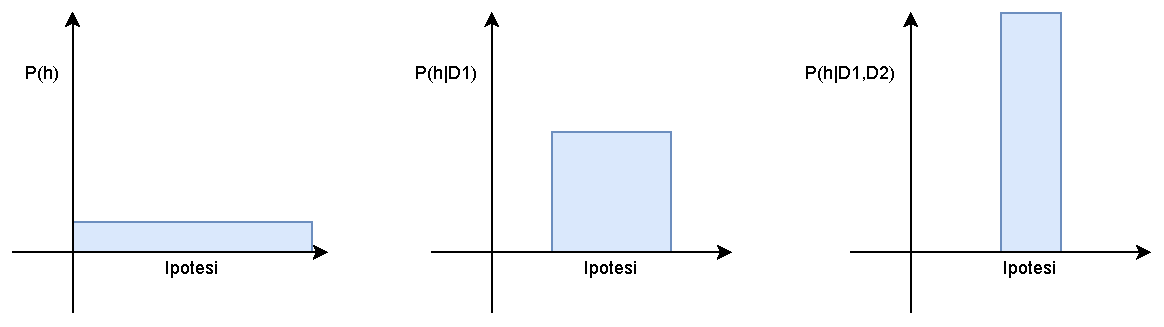
\includegraphics[scale = 0.6]{img/map.pdf}
  \caption{Nell'immagine le evoluzioni di probabilità delle
    ipotesi. Nel primo grafico tutte le ipotesi hanno la stessa probabilità, è
    il punto di partenza. Con gli altri due grafici si ha che man mano che i
    dati di addestramento si accumulano, la probabilità a posteriori delle
    ipotesi inconsistenti diventa zero mentre la probabilità totale che si somma
    a 1 è condivisa equamente tra le ipotesi consistenti rimanenti.}
\end{figure}
Si ha che ogni learner consistente ha in output ipotesi MAP se si assume a
priori la distribuzione uniforme delle probabilità su $H$ dati di training
deterministici e privi di rumore.\\
Riprendendo per esempio anche l'algoritmo find-S si ha che:
\begin{itemize}
  \item ha in output ipotesi consistenti e quindi ipotesi MAP sotto la
  distribuzione di probabilità $P(h)$ e $P(D|h)$
  \item $\forall\,P(h)$ che favorisce le ipotesi più specifiche find-S trova
  appunto le ipotesi MAP
\end{itemize}
A riprova che il metodo Bayesano è un modo per caratterizzare il comportamento
degli algoritmi di apprendimento.\\
inoltre, identificando $P(h)$ e $P(D|h)$ base alle quali l'output è l'ipotesi
ottimale, è possibile caratterizzare le ipotesi implicite dell'algoritmo ovvero
il \textbf{bias induttivo} dell'algoritmo (avendo anche che l'inferenza
induttiva è modellata da un sistema di ragionamento probabilistico equivalente
basato sul teorema di Bayes). \\
Si introduce ora il problema di apprendere funzioni target a valori continui
(reti neurali regressione lineare etc$\ldots$). Si ha che n base a determinate
ipotesi, qualsiasi algoritmo di apprendimento che minimizzi l'errore quadratico
tra l'ipotesi di output e i dati di addestramento, produrrà un'ipotesi
ML. Prepariamo quindi il nostro insieme di assunzioni per il problema:
\begin{itemize}
  \item $h:X\to\mathbb{R},\,\,\,\forall\,h\in H$
  \item li esempi sono della forma $\langle x_i, d_i\rangle$
  \item la funzione target è definita come $f:X\to\mathbb{R}$
  \item si hanno $m$ esempi di training dove il valore target di ogni esempio è
  ``sporcato'' dal rumore casuale $e_i$ secondo una distribuzione di probabilità
  normale con media nulla, avendo $d_i=f(x_i)+e_i$
\end{itemize}
Avendo quindi che $h_{ML}=\operatorname*{argmax}_{h\in H}P(D|h)$ e che gli
eventi di training vengono assunti come indipendenti si ha che:
\[h_{ML}=\operatorname*{argmax}_{h\in H}\prod_{i=1}^mP(d_i|h)\]
Dato quindi l'errore e$_i$ distribuito normalmente con media zero e varianza
sconosciuta $\sigma^2$ si ha che anche ogni $d_i$ segue la stessa
distribuzione attorno al target $f(x_i)$. Poiché stiamo scrivendo l'espressione
per $P(D|h)$, assumiamo che $h$ sia la descrizione corretta per $f$, quindi:
\[\mu=f(x_i)=h(x_i)\]
e avendo quindi, per la distribuzione normale:
\[h_{ML}=\operatorname*{argmax}_{h\in H}
  \prod_{i=1}^m\frac{1}{\sqrt{2\pi\sigma^2}}
  e^{-\frac{1}{2\sigma^2}(d_i-h(x_i))^2}\]
È comune massimizzare il logaritmo meno complicato, a causa della monotonia di
questa funzione, avendo:
\[h_{ML}=\operatorname*{argmax}_{h\in
    H}\prod_{i=1}^m\frac{1}{\sqrt{2\pi\sigma^2}}
  -\frac{1}{2\sigma^2}(d_i-h(x_i))^2\]
ma il primo termine è costante e indipendente da $h$ e quindi può essere
cancellato:
\[h_{ML}=\operatorname*{argmax}_{h\in
    H}\prod_{i=1}^m -\frac{1}{2\sigma^2}(d_i-h(x_i))^2\]
Sapendo che massimizzare questo termine negativo equivale a ridurre al minimo il
termine positivo corrispondente:
\[h_{ML}=\operatorname*{argmin}_{h\in
    H}\prod_{i=1}^m \frac{1}{2\sigma^2}(d_i-h(x_i))^2\]
e avendo che anche tutte le costanti sono indipendenti da $h$ e quindi possono
essere rimosse:
\[h_{ML}=\operatorname*{argmin}_{h\in H}\prod_{i=1}^m (d_i-h(x_i))^2\]
trovando che $h_{ML}$ è ciò che minimizza gli errori quadratici. \\
Si specifica la scelta della normale in quanto:
\begin{itemize}
  \item buona approssimazione di molti tipi di rumore nei sistemi fisici 
  \item il Teorema del Limite Centrale mostra che la somma di un numero
  sufficientemente grande di variabili casuali indipendenti e identicamente
  distribuite obbedisce a una distribuzione Normale 
\end{itemize}
\textbf{\textit{Si considera solo il rumore sul valore del target e non sugli
    attributi che descrivono le istanze stesse}}.\\
Anche in questo caso si usa il Rasoio di Occam, scegliendo di usare il principio
\textbf{Minimum Description Length (\textit{MDL})}, scegliendo la spiegazione
più breve per i dati osservati.\\
Tramite MDL posso ``giustificare'' la scelta di $h_{MAP}$ in base alla teoria
dell'informazione, infatti:
\[h_{MAP}=\operatorname*{argmax}_{h\in H}P(D|h)P(h)\]
\[=\operatorname*{argmax}_{h\in H}\log_2P(D|h)+\log_2P(h)\]
\[=\operatorname*{argmin}_{h\in H}-\log_2P(D|h)-\log_2P(h)\]
e queste equazioni possono essere interpretate come un'affermazione che sono
preferite ipotesi brevi, assumendo un particolare schema di rappresentazione per
la codifica di ipotesi e dati.\\
Il principio MDL fornisce un modo per scambiare la complessità delle ipotesi
per il numero di errori commessi dall'ipotesi.\\

\textbf{Su slide altre informazioni su teoria dell'informazione.}
\section{Classificatore Bayesano ottimo}
Ci si chiede quindi qual è la classificazione più probabile della nuova istanza
secondo i dati di training.\\
Vediamo con un esempio che non basta applicare $h_{MAP}$:
\begin{esempio}
  Sia $H=\{h_1,h_2,h_3\}$ con $P(h_1)=0.4$ e $P(h_2)=P(h_3)=0.3$.\\
  Si ha quindi che:
  \[h_{MAP}=h_1\]
  Consideriamo però una nuova istanza $x$ classificata positiva per $h_1$ e
  negativa per le altre due. Si ha quindi che:
  \begin{itemize}
    \item la probabilità che $x$ sia positivo è 0.4
    \item la probabilità che $x$ sia negativo è 0.6
  \end{itemize}
  e quindi la classificazione più probabile non è quella di $h_{MAP}$.
\end{esempio}
Abbiamo che la classificazione più probabile si ottiene combinando le previsioni
di tutte le ipotesi, ponderate in base alle loro probabilità posteriori. Data
$P(v_j|D)$ come la probabilità che la classificazione corretta sia $v_j$:
\[P(v_j|D)=\sum_{h_i\in H}P(v_j|h_i)P(h_i|D)\]
ottenendo che il classificatore Bayesano ottimo è:
\[\operatorname*{argmax}_{v_j\in V}\sum_{h_i\in H}P(v_j|h_i)P(h_i|D)\]
dato $V$ come insieme dei target (?).
\begin{esempio}
  Vediamo un esempio chiarificatore.\\
  Sia $V=\{+,-\}$ e siano:
  \begin{itemize}
    \item $P(h_1, D) =0.4,\,\,\,P(-, h_1) = 0,\,\,\,P(+, h_1) = 1$
    \item $P(h_2, D) =0.3\,\,\,P(-, h_2) = 1,\,\,\,P(+, h2) = 0$
    \item $P(h_3, D) =0.3,\,\,\,P(-, h_3) = 1,\,\,\,P(+, h3) = 0$
  \end{itemize}
  Si hanno:
  \[\sum_{h_i\in H}P(+|h_i)P)(h_i|D)=0.4\]
  \[\sum_{h_i\in H}P(-|h_i)P)(h_i|D)=0.6\]
  \[\operatorname*{argmax}_{v_j\in \{+,-\}}\sum_{h_i\in H}P(v_j|h_i)P(h_i|D)=-\]
\end{esempio}
\section{Classificatore Bayesano naive}
Il Classificatore Bayesano naive si applica alle attività di learning in
cui ogni istanza $x$ è descritta da una giunzione di valori di attributi e in
cui la funzione target $f(x)$ può prendere un valore qualsiasi dall'insieme
finito $V$. Descriviamo gli esempi di training come $\langle a_1, a_2,\ldots
a_n\rangle $. \\
Applicando il metodo Bayesano si ha:
\[v_{MAP}=\operatorname*{argmax}_{v_j\in V}P(v_j|a_1, a_2,\ldots a_n)\]
\[=\operatorname*{argmax}_{v_j\in V}\frac{P(a_1, a_2,\ldots
    a_n|v_j)P(v_j)}{P(a_1, a_2,\ldots a_n)}\]
e, rimuovendo le i fattori indipendenti:
\[v_{MAP}=\operatorname*{argmax}_{v_j\in V}P(a_1, a_2,\ldots a_n|v_j)P(v_j)\]
Avendo che:
\begin{itemize}
  \item $P(v_j)$ può essere stimato tramite la frequenza di $v_j$ in $D$
  \item $P(a_1, a_2,\ldots a_n|v_j)$ non può essere stimato in questo modo am il
  numero di questi termini è pari a $|X|\cdot |V|$
\end{itemize}
Con il classificatore Bayesano naive si hanno diverse semplificazioni. In primis
i valori degli attributi sono condizionatamente indipendenti comprando:
\begin{itemize}
  \item $P(a_1, a_2,\ldots a_n|v_J)=\prod_iP(a_i|v_j)$
  \item il numero dei termini $a_1, a_2,\ldots a_n$ è pari a:
  \[|DA|\cdot |DT|+|DT|\]
  ove:
  \begin{itemize}
    \item $DA$ sta per attributi distinti/unici
    \item $DT$ sta per valori di target distinti/unici
  \end{itemize}
  \item non si ha la ricerca esplicita dentro $H$ ma solo il contro delle
  frequenze 
\end{itemize}
Si ha quindi il classificatore Bayesano naive:
\[v_{NB}=\operatorname*{argmax}_{v_j\in V}P(v_j)\prod_iP(a_i|v_j)\]
\newpage
\begin{esempio}
  Vediamo un esempio chiarificatore.\\
  Sia dato il seguente dataset, con il target \textit{PlayTennis}:
  \begin{figure}[H]
    \centering
\    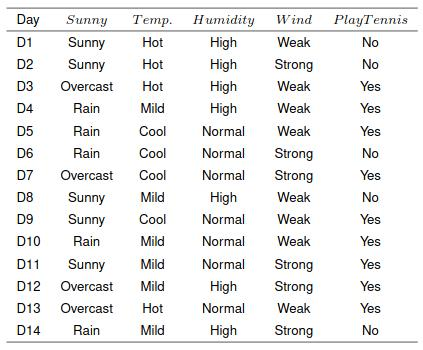
\includegraphics[scale = 0.7]{img/cbn.jpg}
  \end{figure}
  Si ha la nuova istanza:
  \[\langle Outlook=Sunny, Temperature=Cool, Humidity=High,
      Wind=Strong \rangle\]
  Si ha quindi che:
  \[\prod_iP(a_i|v_j)=(Outlook=sunny|v_j)\cdot
      P(Temperature=cool|v_j)\]\[\cdot P(Humidity=high|v_j)\cdot
      P(Wind=strong|v_j)\]
 
  Avendo la stima delle probabilità:
  \[P(PlayTennis=yes)=\frac{9}{14}=0.64\]
  \[P(PlayTennis=no)=\frac{5}{14}=0.36\]
  In modo analogo calcolo le probabilità condizionali. Per esempio per
  $Wing=Strong$:
  \[P(Wing=Strong|PlayTennis=yes)=\frac{3}{9}=0.33\]
  \[P(Wing=Strong|PlayTennis=no)=\frac{3}{5}=0.60\]
  Posso quindi calcolare $v_{NB}$:
  \[P(yes)\cdot P(Sunny|yes)\cdot P(cool|yes)\cdot P(high|yes)\cdot
    P(cool|yes)=0.0053\]
  \[P(yes)\cdot P(Sunny|no)\cdot P(cool|no)\cdot P(high|no)\cdot
    P(cool|no)=0.0206\]
  Quindi si ha che:
  \[v_{NB}=no\]
  e normalizzando:
  \[\frac{0.0206}{0.0206+0.0053}\]
\end{esempio}
Si è visto come, normalmente, le probabilità sono stimate dalla frazione di
volte in cui si osserva che l'evento si verifica sul numero totale di
opportunità $N$:
\[\frac{n_c}{N}\]
è spesso questo metodo fornisce una buona stima.\\
Si ha però un limite se $n_c$ è molto piccolo, avendo risultati errati con:
\begin{itemize}
  \item sottovalutazione delle probabilità a causa di un bias
  \item se addirittura $n_c$ è nullo esso ``dominerà'' sul classificatore
  Bayesano 
\end{itemize}
Si introduce un nuovo approccio Bayesano sfruttando il cosiddetto
\textbf{m-estimate}, ovvero: 
\[\frac{n_c+m\cdot p}{n+m}\]
dove $p$ è una stima precedente della probabilità che desideriamo determinare,
ed $m$ è una costante chiamata \textit{equivalent sample size} che determina
quanto sia importante il peso di $p$ rispetto ai dati osservati.\\
In assenza di informazioni aggiuntive $p$ ha distribuzione uniforme quindi si
ha, per $k$ numero di possibili valori di attributo:
\[p=\frac{1}{k}\]
Si nota che per $m$ nullo si ha che l'm-estimate è uguale a:
\[\frac{n_c}{n}\]
e quindi $m$ può essere interpretato come il numero di campioni virtuali
distribuiti su $p$ a cui vengono aggiunti gli $n$ esempi effettivi osservati.\\
% capire se serve parte su reti
\end{document} 

% LocalWords:  Machine Learning machine learning dataset fit overfitting sse 
% LocalWords:  Concept concept experience learner rewards inductive validation
% LocalWords:  find Find findS version List biased Hypothesis unbiased bias yes
% LocalWords:  bias prover information gain slide level sibling distance wind
% LocalWords:  weak outlook sunny humidity high normal overcast rain branch IG
% LocalWords:  primis True backtracking greedy overfit split Description Length
% LocalWords:  cloudy rainy warm cold sky temp humid forecast same change Venn
% LocalWords:  darkgreen list then example label dell nell refractory Hebb pre
% LocalWords:  McCulloch Pitts sigmoide Percettrone percettroni iperpiano error
% LocalWords:  function Papert Minsky perceptron Recall feedforward layer Unit
% LocalWords:  Linear Treshold LTU soddisfacibilità replace percettrone ALVINN
% LocalWords:  retropropagazione nodes branches leef outcome pdf red Shannon VC
% LocalWords:  Support Vector Machines SVM Machines Vector Support LocalWords
% LocalWords:  iperpiani Cervonenkis Vapnik support vector kernel trick Bayes
% LocalWords:  riscalato Bayesano
